\documentclass[conference]{IEEEtran}
\IEEEoverridecommandlockouts
% The preceding line is only needed to identify funding in the first footnote. If that is unneeded, please comment it out.
\usepackage{cite}
\usepackage{amsmath,amssymb,amsfonts}
\usepackage{algorithmic}
\usepackage{booktabs}
\usepackage{graphicx}
\usepackage{textcomp}
\usepackage{xcolor}
\usepackage{natbib}
\usepackage{url}
\usepackage{hyperref}
\usepackage{subcaption}


\def\BibTeX{{\rm B\kern-.05em{\sc i\kern-.025em b}\kern-.08em
    T\kern-.1667em\lower.7ex\hbox{E}\kern-.125emX}}
\graphicspath{{images/}}

\begin{document}

\title{Armenian Speech-to-Text Recognition\\
\textit{Spring 2024}}

% \author{\IEEEauthorblockN{\textit{Tigran Gaplanyan, Sanasar Hambardzumyan, Anahit Baghdasaryan}}
% \IEEEauthorblockA{Supervisor: \textit{Elen Vardanyan} \\
%  {American University of Armenia}\\
% }
% }

\author{\IEEEauthorblockN{Tigran Gaplanyan}
\IEEEauthorblockA{\textit{BS in Computer Science} \\
\textit{American University of Armenia}}
\and
\IEEEauthorblockN{Sanasar Hambardzumyan}
\IEEEauthorblockA{\textit{BS in Computer Science} \\\textit{American University of Armenia}
\and
\IEEEauthorblockN{Anahit Baghdasaryan}
\IEEEauthorblockA{\textit{BS in Data Science} \\\textit{American University of Armenia}}
\and
\IEEEauthorblockN{Supervisor: Elen Vardanyan}
\IEEEauthorblockA{\textit{American University of Armenia}}
}}

\maketitle

\begin{abstract}
This project aims to address the need for Speech-to-Text Recognition (STR) technology in the Armenian language by creating a practical and efficient system. Leveraging pre-trained Automatic Speech Recognition (ASR) models, the project fine-tunes them using the latest releases (16.1 and 17.0) of the Common Voice Armenian Audio Dataset. Through a sophisticated ecosystem comprising frontend and backend components integrated with MongoDB for data management and hosted on a cloud-based server, the project aims to deliver a practical and efficient web app. The web app offers users a user-friendly platform to experiment with different speech recognition models, such as Whisper, Vaw2Vec2, Quartznet, Citrinet, and more, to transcribe audio recordings and manage their transcription history. Through a comprehensive account of the development process, including encountered challenges and implemented solutions, this project seeks to advance the field of speech-to-text recognition while advocating for the integration of the Armenian language into modern digital communication.
\end{abstract}

\section{Introduction}

The Armenian language has a rich historical background and is considered one of the earliest branches of the Indo-European language family. It has persisted into written history, yet the technological advancements, specifically in the Speech-to-Text Recognition (STR) domain, have not fully embraced the linguistic nuances of Armenian. This gap in technological representation has provoked the initiation of this project, aimed at creating a practical and efficient Speech-to-Text Recognition system specifically for the Armenian language.

In response to this imperative, our project attempts to not only address the existing deficiency but also contribute to the further advancement of Armenian speech recognition technology. By utilizing the latest Automatic Speech Recognition (ASR) models and the latest (16.1 and 17.0) Common Voice Armenian Audio Datasets, we aspire to conduct a comparative experiment by fine-tuning different ASR models and achieving higher accuracy in transcribing Armenian audio data. Furthermore, central to our endeavor is developing a web app that offers a user-friendly platform to experiment with fine-tuned speech recognition models such as Whisper, Vaw2Vec2, Quartznet, Citrinet, etc.

The following methodology was primarily employed in the scope of our project.

\begin{itemize}
    \item \textbf{Exploration of Common Voice 16.1 and 17.0 Armenian Dataset:} In this initial phase, we delved into the Common Voice 16.1 and 17.0 Armenian Datasets to understand their structure, content, and quality. This step was crucial for identifying the data preprocessing requirements and selecting appropriate ASR models for fine-tuning.
    \item \textbf{Preprocessing of Dataset for ASR Model Compatibility:} Following dataset exploration, we conducted preprocessing typical to the selected ASR model's specifications: this involved data formatting and more to enhance the dataset's suitability for training the ASR models.
    \item \textbf{Fine-tuning of ASR Models:} Leveraging the preprocessed dataset, we proceeded to fine-tune various ASR models. This iterative process involved training the models on the Armenian dataset to adapt them to the language's specific phonetic and linguistic characteristics.
    \item \textbf{Evaluation using WER and CER Metrics:} To assess the performance of the fine-tuned ASR models, we employed Word Error Rate (WER) and Character Error Rate (CER) metrics. These metrics provided quantitative insights into the accuracy and effectiveness of the models in transcribing Armenian speech.
    \item \textbf{Integration with Web Application:} Upon achieving satisfactory performance levels, we integrated the checkpoints of the fine-tuned ASR models with the web application. This integration enabled users to access the ASR functionality directly through the user-friendly interface of the web application.
    \item \textbf{Front-End Implementation:}
        \begin{itemize}
            \item The React.js framework was used for front-end development.
            \item Created a UI that is easy to use and familiar to users, using inspiration from ChatGPT and similar platforms.
            \item Elements to facilitate smooth user interaction include the Home, Login, Registration, My Transcriptions, and Services pages.
            \item Included necessary libraries, such as React-Spinners for loading animations and Axios for HTTP queries.
            \item Used Vercel for front-end cloud deployment.
        \end{itemize}
        \item \textbf{Back-End Implementation:}
        \begin{itemize}
            \item Java was used to develop the backend and the Spring Boot framework because of its scalability and resilience.
            \item The layered architectural design was used to guarantee maintainability and modularity.
            \item We implemented a repository layer for database access, a service layer for business logic, and controllers to handle incoming requests.
            \item MongoDB was integrated with the application using Spring Boot Starter Data MongoDB, allowing for adequate data storage and retrieval.
        \end{itemize}
    \item \textbf{MongoDB Integration:}
    \begin{itemize}
        \item Database schemas were created to effectively store conversation data, audio file metadata, and user information.
        \item Used the document-based structure of MongoDB to store and handle data in a schema-less setting.
    \end{itemize}
    \item \textbf{Cloud Deployment:}
    \begin{itemize}
        \item Explored best-suited cloud providers for hosting back-end servers.
        \item Opted for Azure, configuring a virtual machine with 16GB RAM and 4v CPUs for deploying the web app.
    \end{itemize}
\end{itemize}

This paper walks you through the detailed sections to better understand each of the components of our methodology, while an extensive literature review spanning from 2016 to 2024, providing unique insights, methodologies, and advancements in the field, creates a bigger image for you. 

\section{Literature Review}

The development of Armenian Speech-to-Text Recognition (ASR) systems has made significant progress in recent years, driven by a growing interest in developing innovative systems for under-resourced languages like Armenian. This section reviews distinct works spanning from 2016 to 2024, each providing unique insights, methodologies, and advancements in the field. These works underscore the challenges and suggest solutions for pursuing accurate and efficient Armenian ASR systems.

\subsection{"Noise-Robust Speech Recognition System for Armenian Language"\cite{author2023noise}} 
Our review begins with Anahit Vardanyan's master's thesis, "Noise-Robust Speech Recognition System for Armenian Language," at the American University of Armenia in 2016. The building blocks included training an acoustic model, generating a dictionary, building grammar, and developing an Android application. The author notes that the quality of the acoustic model is highly dependent on the quality and quantity of the training data and that it is essential to use a diverse and representative dataset to ensure good performance. Furthermore, the ASR system uses a dictionary (a list of words and their corresponding phonetic transcriptions) to map the acoustic signal to a sequence of words and grammar (a set of rules that define the structure of the language and the possible sequences of words) to constrain the search space and improve recognition accuracy. The author states that the testing audio set was segmented into clean, noisy speech samples collected from three speakers, one male and two females. Key findings of the thesis show that the ASR system worked reasonably well on clean speech, but its performance degraded in the presence of noise. 

\begin{table}[h]
    \centering
    \caption{Word Error Rate (\%) for the Testing Audio Set}
    \label{tab:wer_database}
    \begin{tabular}{lcc}
        \toprule
        \textbf{Testing set}: & \textbf{clean speech} & \textbf{noisy speech} \\
        \midrule
        \textbf{Speaker1} (trainer, female, age 24) & 25.3\% (16/63) & 82.8\% (58/70) \\
        \textbf{Speaker2} (female, age 23) & 54.6\% (41/75) & 87.5\% (35/40) \\
        \textbf{Speaker3} (male, age 24) & 62.0\% (54/87) & 97.5\% (39/40) \\
        \midrule
    \end{tabular}
\end{table}


\subsection{"A Conformer-Based Automated Speech Recognition for the Armenian Language" \cite{Karamyan_Davit_A}}
Successively, the research paper "A Conformer-Based Automated Speech Recognition for the Armenian Language" was authored by Davit Karamyan and Tigran Karamyan in February 2022. The paper's key finding demonstrates the effectiveness of the parallel usage of the fine-tuned Conformer-CTC-Medium model pre-trained on the NeMo ASRSET dataset for voice recognition and a compact Armenian language model for text symbol generation. The primary dataset used for the research was "Stories-15," which consisted of about 40 stories in Armenian with 12 readers, totaling to 15 hours. Additionally, half of the audio data from Mozilla Common Voice, specifically version 9.0, was incorporated, totaling to 4 hours, with 60 readers. The evaluation was based on the Word Error Rate (WER) metric, which is discussed more in-depth in the EVALUATION METRICS AND RESULTS section of this paper. The WER for the Conformer-CTC model alone, without any language model, was 68\%, significantly improving to 37\% by incorporating a 10-gram language model. 

\subsection{"Towards a Unified ASR System for the Armenian Standards" \cite{chakmakjian-wang-2022-towards}}
The paper "Towards a Unified ASR System for the Armenian Standards" by Chakmakjian and Wang, published in June 2022, explores the challenges and proposes a methodology for developing an ASR system for the Armenian language, including its two standard branches: Standard Eastern Armenian (SEA) and Standard Western Armenian (SWA). Despite their phonetic and phonological differences, the authors argue for a unified ASR system due to shared writing and vocalic systems, base lexicons, and high mutual intelligibility among proficient speakers. They propose a methodology for creating a unified ASR system, suggesting approaches like grapheme-to-phoneme (G2P) conversion and discriminating between similar languages (DSL) to determine the variant being spoken. While acknowledging a slight performance gap between end-to-end (E2E) ASR systems and hybrid models, the authors believe the upcoming innovations will bridge this gap. 

\subsection{"ArmSpeech: Armenian Spoken Language Corpus" \cite{Melikian2022ArmSpeechAS}}
Moreover, Varuzhan Baghdasaryan's ArmSpeech corpus, presented in May - June 2022, represents a significant contribution to the Armenian ASR research field, providing a rich dataset of annotated Armenian speech addressing the critical need for high-quality training data. The corpus contains 6206 audio samples, which amounts to 11.77 hours of annotated native Armenian speech (62.37\% male and 37.63\% female). This multi-speaker speech corpus consists of 14 sections. The first 13 sections consist of open-source fiction audiobooks, while the 14th section contains speeches covering various real-life scenarios. The audio recordings are provided in mono-channel 16-bit format, with a sampling rate of 16 kHz and a bit rate of 256 kbps, distributed in the lossless compression WAV format. 

\subsection{"Extended ArmSpeech: Armenian Spoken Language Corpus" \cite{Baghdasaryan2022ExtendedAA}}
Further expanding the ArmSpeech project, Baghdasaryan published the "Extended ArmSpeech: Armenian Spoken Language Corpus" paper in July - August 2022. The extended version of ArmSpeech is based on the principle of volunteer voice donation. Recording materials were collected from Armenian news websites' articles about lifestyle, culture, sports, and politics. The extension materials were recorded by native Armenian speakers, specifically, one female (36.31\% of the speeches) and three males (63.69\% of the speeches). The ArmSpeech extended version contains 5378 high-quality annotated audio clips totaling 4 hours, making the total duration of the ArmSpeech corpus 15.7 hours.

\subsection{"Armenian Speech Recognition System: Acoustic and Language Models" \cite{author2023armenian}}
Continuing the research, Baghdasaryan published the paper "Armenian Speech Recognition System: Acoustic and Language Models" in September - October 2022. Baghdasaryan aims to develop acoustic and language models for the Armenian language that can run in real time and perform speech-to-text tasks on IoT devices. The methodology used in the paper involves training the acoustic and language models separately and then combining them to achieve higher accuracy in ASR. The acoustic model defines the relationship between an audio signal and the phonemes, while the language model defines the relationship between words and their sequences. The author used RNN-based Baidu's Deep Speech neural network and the KenLM toolkit to train the probabilistic n-gram language model. The Deep Speech acoustic model was trained and validated on the ArmSpeech corpus and tested on the Common Voice Armenian corpus. The author reports 0.902565 WER / 0.305321 CER for the acoustic model standalone and 0.552975 WER / 0.285904 CER with the language model.

\subsection{"Exploring Armenian Speech Recognition: A Comparative Analysis of ASR Models - Assessing DeepSpeech, Nvidia NeMo QuartzNet, and Citrinet on Varied Armenian Speech Corpora" \cite{inproceedings}}
In September 2023, Baghdasaryan published the paper, "Exploring Armenian Speech Recognition: A Comparative Analysis of ASR Models - Assessing DeepSpeech, Nvidia NeMo QuartzNet, and Citrinet on Varied Armenian Speech Corpora." The paper's primary objective is to evaluate and enhance the accuracy of Armenian speech recognition by comparing three prominent ASR models - DeepSpeech, Nvidia NeMo QuartzNet, and Citrinet. The methodology employed involves a comprehensive evaluation of the three ASR models using three high-quality Armenian speech corpora - ArmSpeech (15.7 hours), Speech corpus of Armenian question-answer dialogues (8.5 hours), and Google's FLEURS (12 hours). The merged dataset combines these three corpora with a random division into training, validation, and testing subsets, maintaining a ratio of 60-20-20\%, respectively. The results, summarized in Table 2 \ref{tab:asr_comparison}, reveal the performance of DeepSpeech, QuartzNet, and Citrinet in terms of size and error rates.

\begin{table}[htbp]
\centering
\caption{Comparison of ASR Models}
\label{tab:asr_comparison}
\begin{tabular}{@{}lccc@{}}
\toprule
\textbf{Model} & \textbf{DeepSpeech} & \textbf{QuartzNet} & \textbf{Citrinet} \\ \midrule
\textbf{Size (MB)} & 180 & 37.87 & 72.73 \\
\textbf{WER/CER with LM} & 0.3231/0.1259 & 0.2676/0.1092 & 0.0869/0.0372 \\
\textbf{WER/CER without LM} & 0.6302/0.1435 & 0.3351/0.1537 & 0.1941/0.0826 \\ \bottomrule
\end{tabular}
\end{table}

\subsection{"Enhancing Armenian Automatic Speech Recognition Performance: A Comprehensive Strategy for Speed, Accuracy, and Linguistic Refinement" \cite{baghdasaryan2024enhancing}}
As a final note, Baghdasaryan's 2024 paper "Enhancing Armenian Automatic Speech Recognition Performance: A Comprehensive Strategy for Speed, Accuracy, and Linguistic Refinement" outlines a comprehensive strategy to improve the performance of the previously built Armenian ASR system. The primary objectives are to update the previously fine-tuned Citrinet model with new datasets, optimize its speed and efficiency for near real-time processing, and enhance the linguistic quality of transcriptions by introducing punctuation and capitalization. Therefore, the model was updated with samples from the Common Voice corpus and data anonymously collected via the armspeech.com web application. Hence, Citrinet accomplished a WER of 13.4\%, notably bypassing the model's previous performance of (19.41\%). Moreover,  the model's architecture underwent a reduction, resulting in a lighter model and reducing both training and recognition durations. Although this adjustment caused a slight increase in the WER to 18.2\%, the time taken for speech recognition experienced an average decrease of 26\%. Finally, a punctuation and capitalization model, utilizing the Transformer Distilbert architecture, was developed to enhance the ASR output, guaranteeing readability, usability, and grammatical accuracy.


In conclusion, this section showcased a dynamic and evolving landscape of Armenian ASR research, characterized by innovative methodologies, diverse datasets, and a growing interest in linguistic diversity in technology development. These works collectively contribute to the advancement of Armenian ASR systems, laying the foundation for future innovations in the field.

\section{Tools}

\subsection{Whisper: An Automatic Speech Recognition System}

\quad \quad An automated speech recognition (ASR) system called Whisper was trained using web-sourced, 680,000 hours of multilingual, multitask supervised data. The robustness against accents, background noise, and technical terminology is enhanced by the utilisation of such a huge and diversified dataset. Additionally, it facilitates translation into English from other languages as well as multilingual transcription.

The encoder-decoder Transformer is the implementation of the straightforward end-to-end Whisper architecture. The audio input is divided into 30-second segments, transformed into a log-Mel spectrum, and subsequently fed into an encoder. In order to train a single model to do tasks like multilingual voice transcription, phrase-level timestamps, language identification, and to-English speech translation, a decoder is trained to predict the matching text caption, mixed with special tokens (see in Figure 1).

Approximately one-third of Whisper's audio dataset is non-English, and it is assigned the task of transcribing in the original language or translating to English.

Unlike a considerable amount of work on voice recognition, Whisper models learned to map statements to their transcribed form based on the expressiveness of sequence-to-sequence models, and were trained to predict the raw text of transcripts without significant standardisation. Audio from the Internet was combined with transcripts to create the pre-training dataset. As a result, there is an extensive variety of audio from various settings, recording configurations, speakers, and languages in the collection. Diversity in text quality is not as beneficial as diversity in audio quality when it comes to training a robust model. Several automated filtering techniques have been developed to increase transcript quality in order to overcome this.

An 80-channel log- magnitude Mel spectrogram representation is created on 25-millisecond windows with a stride of 10 milliseconds once all audio has been re-sampled to 16,000 Hz.The input was scaled to be between -1 and 1, with a mean of roughly zero across the pre-training dataset for further  normalisation. The encoder works with thefollowing specifications: with a tiny stem made up of two convolution layers with a filter width of three and the GELU activation function-the second convolution layer having a stride of two. The encoder Transformer blocks are applied once sinusoidal position embeddings have been added to the stem's output.

Pre-activation residual blocks are used in the transformer, and the encoder output is subjected to a final layer normalisation. Tied input-output token representations and learned position embeddings are put to use by the decoder. The width and quantity of transformer blocks are identical between the encoder and decoder.

\begin{figure*}[ht]
\centering
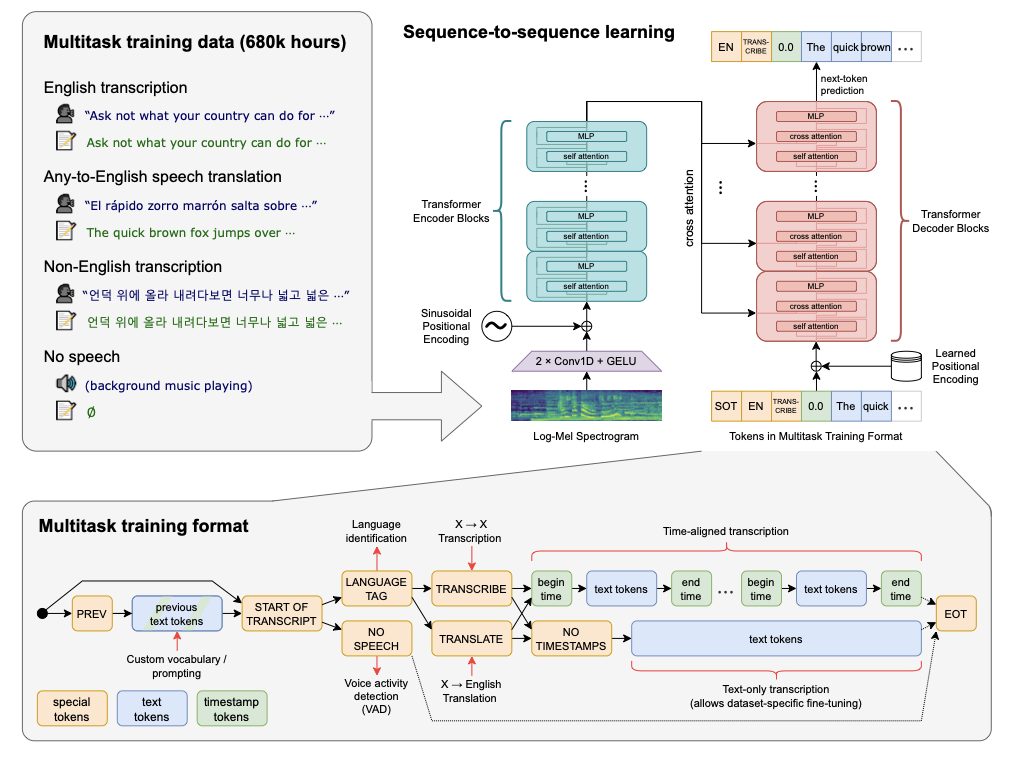
\includegraphics[width=\textwidth]{1.png}
\caption{\textbf{Overview of approach.} In multilingual speech recognition and translation, spoken language identification and voice activity detection, the sequence to sequence Transformer model was trained. The decoder is able to forecast these tasks together by representing them as a sequence of tokens that need to be predicted once.
Thus, for traditional speech processing pipeline, a single model can substitute many different stages.}
\label{fig:whisper_asr_architecture}
\end{figure*}

For the English-only models, the same byte-level BPE text tokenizer as in GPT-2 was used. For the multilingual models, the vocabulary was modified while maintaining the same size to prevent excessive decomposition on other languages, as the GPT-2 BPE vocabulary is limited to English. The decoder, an audio-conditional language model, was trained to learn how to resolve ambiguous audio by using longer-range text context based on the transcript's text history. The model learned to predict all other tokens by masking only the training loss over the prior context text.


The idea of training the models of different sizes was to examine Whisper's scalability characteristics. FP16 with dynamic loss scaling and activation check-pointing was used for training with data parallelism across accelerators. AdamW and gradient norm clipping were used to train the models, with a linear learning rate decaying to zero after a warmup over the first 2048 updates. A batch size of 256 segments was chosen, and the models were trained for 220 updates, which corresponds to two to three passes over the dataset. Overfitting is not a major concern because the model was only trained for a small number of epochs. Moreover, no regularisation or data augmentation was applied; instead, generalisation was encouraged by the variety present in such a huge dataset.

\begin{table}[ht]
\centering
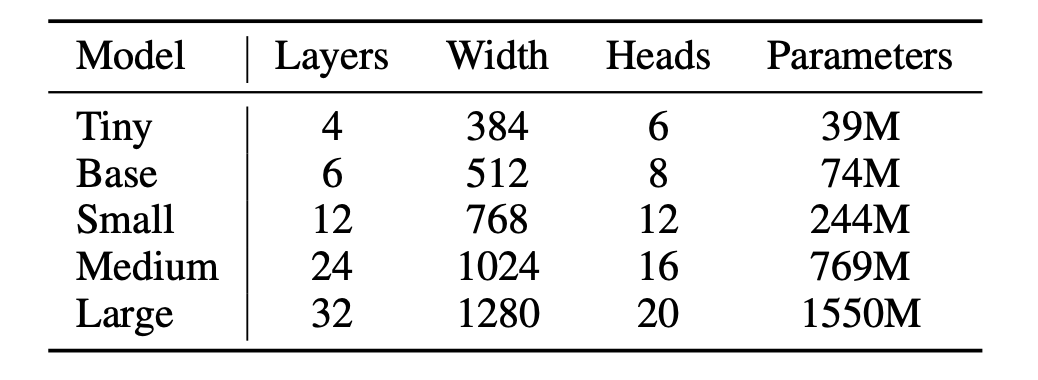
\includegraphics[width=0.5\textwidth]{2.png}
\caption{Architecture details of the Whisper model family.}
\label{fig:whisper_asr_architecture}
\end{table}

Instead of utilising the typical evaluation technique for these datasets, which includes both a train and test split, Whisper was assessed in a zero-shot condition with no training data for each trained dataset, allowing for extensive generalisation of evaluation. In speech recognition research, the word error rate (WER) statistic is commonly used to assess and compare systems. Before the WER computation, the text was heavily standardised in order to reduce the penalization of non-semantic discrepancies. \cite{radford2022}

\subsection{Wav2vec Framework}

\quad \quad Wav2vec is utilised to learn representations from unprocessed audio data on its own. A multi-layer convolutional neural network is used in the model to encode speech audio. Similar to masked language modelling, spans of the generated latent speech representations are then masked. In order to create contextualised representations, the latent representations are loaded into a Transformer network. The model is then trained using a contrastive task in which the true latent has to be identified from distractions.

To capture the latent representations in the contrastive task, the model learned discrete speech units during training using a gumbel softmax. In order to employ the model for downstream speech recognition tasks, it is pre-trained on unlabeled speech data and then refined on labelled data using a Connectionist Temporal Classification (CTC) loss.

The model is composed of a multi-layer convolutional feature encoder \( f : X^7 \rightarrow Z \) which takes as input raw audio X and outputs latent speech representations \( z_1, \ldots, z_T \) for T time-steps. They are then fed to a Transformer \( g:Z^7 \rightarrow C \) to build representations \(c_1,\ldots,c_T\) capturing information from the entire sequence. The output of the feature encoder is discretized to \(q_t\) with a quantization module \( Z^7 \rightarrow Q \) to represent the targets (Figure 2) in the self-supervised objective.

\begin{figure}[ht]
\centering
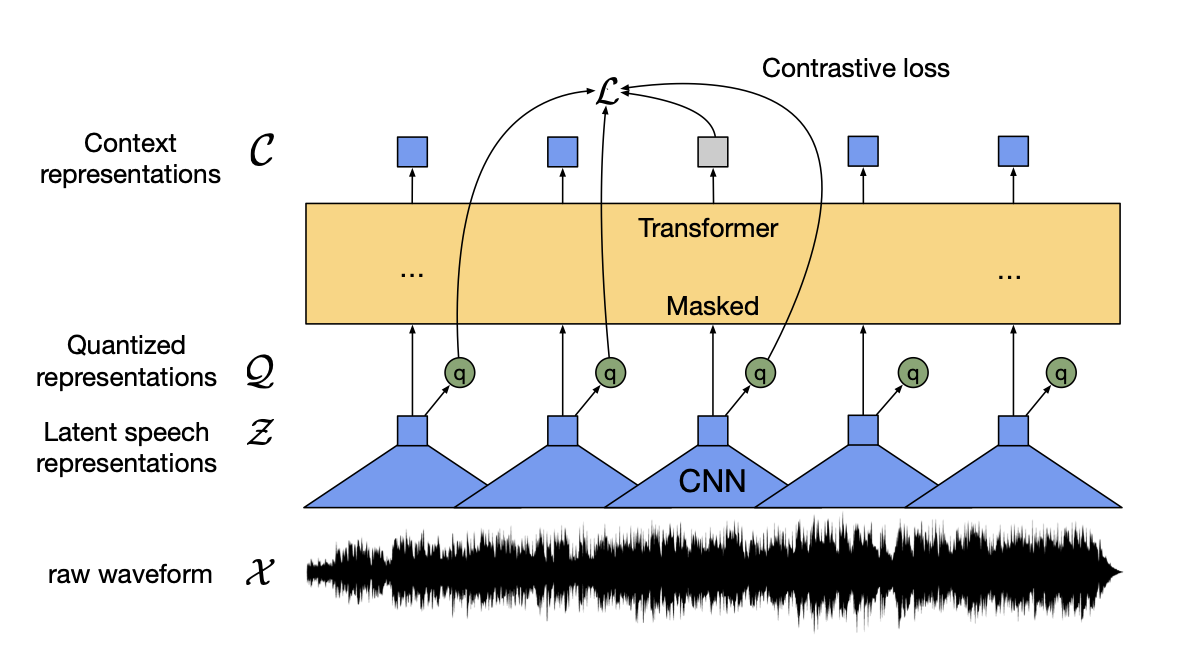
\includegraphics[width=0.5\textwidth]{15.png}
\caption{Illustrating the structure learning contextualized discourse representations and a repository of quantified speech units}
\label{fig:whisper_asr_architecture}
\end{figure}

A temporal convolution, layer normalisation, and a GELU activation function are the blocks that make up the encoder. The encoder normalises the unprocessed waveform input to zero mean and unit variance. The amount of time-steps T that are entered into the Transformer is set by the encoder's total stride.

The Transformer architecture-based context network receives the feature encoder's output. Convolutional layer, which functions as a relative positional embedding, was utilised in place of fixed positional embeddings, which encode absolute positional information. The convolution's output is then added to the inputs, and layer normalisation is applied after a GELU. \cite{baevski2020}

\subsection{SeamlessM4T Model}

\quad \quad SeamlessM4T is a multitask and multilingual model, which trancribes and translates both text and speech without any interruption. It recognizes, translates speech-to-text, text-to-text for approximately 100 languages. Moreover, it translates speech-to-speech, text-to-speech for about 100 input languages and 35 output languages including English.

The multitask UnitY model architecture, which can produce translated text and speech directly, was employed for the model. It enables automatic speech recognition, text-to-text, text-to-speech, speech-to text, and speech-to-speech translations. There are three primary sequential components that comprise the multitask UnitY model. Text and speech encoder is able to recognize speech input for almost 100 languages. After that, the text decoder converts the meaning into almost 100 different languages for text. For 36 spoken languages, it decodes the meaning into discrete acoustic units. Pre-training the self-supervised encoder, speech-to-text, text-to-text translation components, and text-to-unit model enhances the model's quality and ensures training stability. After the discrete units are decoded, a multilingual HiFi-GAN unit vocoder is used to translate them into voice (see in Figure 3).

\begin{figure}[ht]
\centering
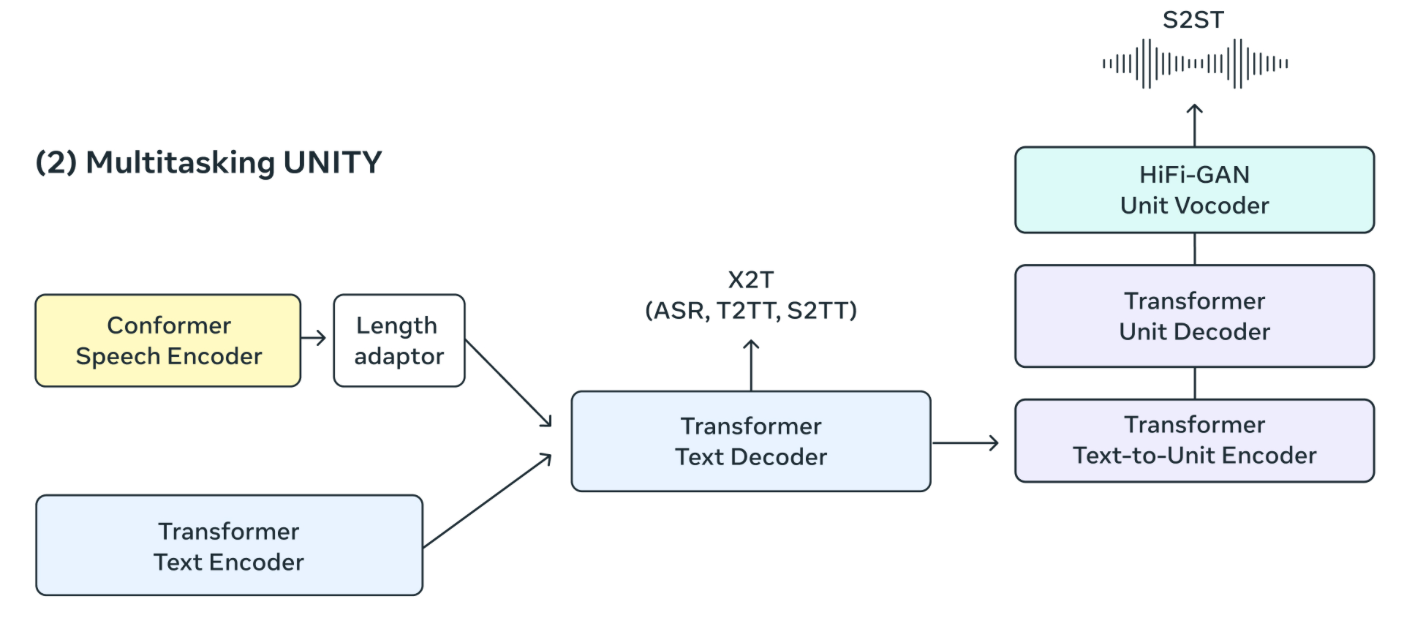
\includegraphics[width=0.5\textwidth]{16.png}
\caption{Multitasking UNITY}
\label{fig:whisper_asr_architecture}
\end{figure}

W2v-BERT 2.0, a self-supervised speech encoder, gains the ability to comprehend speech by examining millions of hours of multilingual speech. After decomposing the audio stream into smaller components, the encoder creates an internal representation of speech. Many of those sounds and characters are found in spoken words, thus a length adaptor was employed to roughly transform them to actual words. The text encoder has been taught to comprehend text in approximately 100 languages and provide translational representations.

It is possible for the text decoder to accept either text or encoded speech representations. Applications for this include multilingual translation and tasks involving automatic speech recognition in the same language. Through multitask training, the speech-to-text translation model was guided by token-level knowledge distillation, utilising the strengths of a robust text-to-text translation model (NLLB).

To depict speech on the target side, acoustic units were employed. The UnitY model's text-to-unit (T2U) component, which is pre-trained on ASR data before UnitY fine-tuning, creates these discrete speech units based on the text output. Following that, these discrete units are transformed into audio waveforms using a multilingual HiFi-GAN unit vocoder.

Performance for supported low and mid-resource languages has also greatly improved, while good performance for high-resource languages is maintained. \cite{barrault2023}

\subsection{Microsoft Azure Service}

\quad \quad The speech recognition technology from Microsoft Azure takes advantage of the latest developments in cloud computing and machine learning to provide reliable and expandable solutions.
Azure's voice recognition model is based on a deep neural network architecture, which is optimised for speed and accuracy in a wide range of languages and dialects. Azure's speech recognition engine is based on a Universal Language Model. Pre-trained on data held by Microsoft, this model captures a broad range of phonetics and dialects common to a language. Azure supports custom model integration for certain tasks. To improve the base model's identification performance, these customised models are trained using audio instances and vocabulary unique to the domain. \cite{microsoftnd}

Microsoft Research's latest developments are driving automated speech recognition (ASR) towards end-to-end (E2E) models. The integration of all speech recognition components into a single model, known as E2E models, streamlines the training process and may increase recognition accuracy. These models can be customised for certain domains, have low latency, and accommodate multilingual users. \cite{li2021}

\subsection{QuartzNet}

The QuartzNet model by NVIDIA NeMo\cite{9053889} is a novel end-to-end neural acoustic model designed for automatic speech recognition (ASR). This model is composed of multiple blocks with residual connections between them, where each block consists of one or more modules with 1D time-channel separable convolutional layers, batch normalization, and ReLU layers. 

The motivation behind developing the QuartzNet model is to build an ASR model that achieves state-of-the-art-level accuracy while utilizing significantly fewer parameters and less computing power. The model is trained with CTC loss and achieves near state-of-the-art accuracy/WER on LibriSpeech and Wall Street Journal datasets, with fewer than 20 million parameters, compared to previous end-to-end ASR designs, which typically have over 100 million parameters. The best results on the LibriSpeech dataset are achieved with the QuartzNet-15x5 model, consisting of 15 blocks with 5 convolutional modules per block. By combining the network with independently trained language models, the model achieves WER comparable to the current state-of-the-art. 

The QuartzNet model alone achieves near state-of-the-art accuracy/WER  by building a very deep neural network with 1D time-channel separable convolutions. The QuartzNet model's architecture is based on the Jasper architecture, a convolutional model trained with Connectionist Temporal Classification (CTC) loss. The main novelty in QuartzNet's architecture is the replacement of 1D convolutions with 1D time-channel separable convolutions, an implementation of depthwise separable convolutions. 1D time-channel separable convolutions can be separated into a 1D depthwise convolutional layer with kernel length K that operates on each channel individually but across time frames and a pointwise convolutional layer that operates on each time frame independently but across all channels.

The QuartzNet models have the following structure: they start with a 1D convolutional layer C\textsubscript{1} followed by a sequence of blocks. Each block B\textsubscript{i} is repeated S\textsubscript{i} times and has residual connections between blocks . Each block B\textsubscript{i} consists of the same base modules repeated R\textsubscript{i} times and contains four layers:
\begin{itemize}

\item A K-sized depthwise convolutional layer with cout channels
\item A pointwise convolution
\item A normalization layer
\item ReLU

\end{itemize}

The last part of the model consists of three additional convolutional layers (C\textsubscript{2}, C\textsubscript{3}, C\textsubscript{4}). The C\textsubscript{1} layer has a stride of 2, and the C\textsubscript{4} layer has a dilation of 2. 

\begin{figure}[ht]
\centering
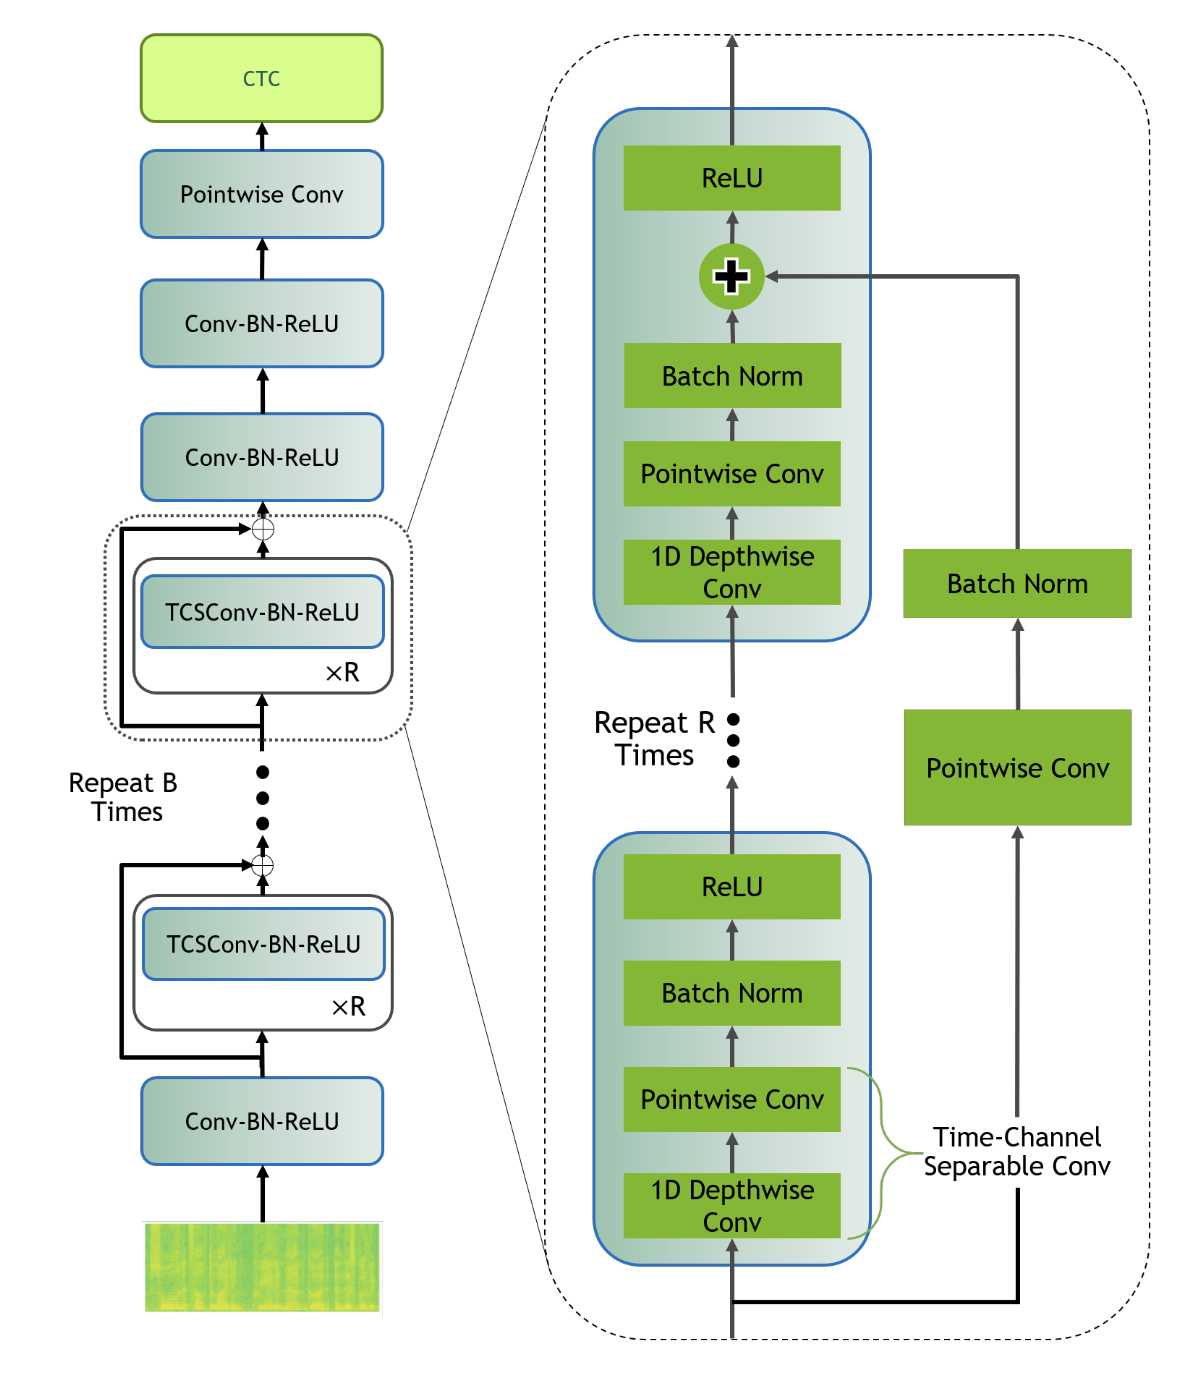
\includegraphics[width=0.5\textwidth]{QuartzNet.png}
\caption{QuartzNet BxR architecture}
\label{fig:QuartzNet_asr_architecture}
\end{figure}

To further reduce the number of parameters, the model explores using group convolutions for the pointwise convolution part. A group shuffle layer is also added to increase cross-group interchange. Using groups allows for a significant reduction in the number of weights at the cost of some accuracy.

Since the model is much smaller than a model with regular convolutions, it is less prone to overfitting. Therefore, only data augmentation and weight decay are used for regularization during training. 


\subsection{Citrinet\cite{Majumdar2021CitrinetCT}}

Citrinet by NVIDIA NeMo is a novel end-to-end convolutional Connectionist Temporal Classification (CTC) based automatic speech recognition (ASR) model. The model aims to bridge the gap between non-autoregressive and autoregressive end-to-end ASR models. Citrinet is a deep residual neural model that employs 1D time-channel separable convolutions combined with sub-word encoding and squeeze-and-excitation.

The Citrinet encoder combines 1D time-channel separable convolutions from QuartzNet with the squeeze-and-excitation (SE) mechanism from ContextNet. This combination of architectural elements significantly allows Citrinet to close the gap between CTC and the best Seq2Seq and Transducers models. The model achieves competitive performance on various speech recognition datasets, including LibriSpeech, TED-LIUM 2, AISHELL-1, Multilingual LibriSpeech, etc.

The paper "Citrinet: Closing the Gap between Non-Autoregressive and Autoregressive End-to-End Models for Automatic Speech Recognition" presents experimental results on the LibriSpeech dataset using five configurations of Citrinet with different numbers of channels C. The models are trained using the NovoGrad optimizer with a learning rate of 0.05, $\beta_1 = 0.8$, $\beta_2 = 0.25$, and weight decay 0.001. SpecAugment is used for data augmentation. The results show that Citrinet performs competitively compared to Transducers such as ContextNet and Conformer. The largest Citrinet model achieves a greedy WER of 6.2\% on the test-other set, and with LM rescoring, the gap between Citrinet and SOTA Transducers for test-other is reduced to only 0.59-0.79\%

The Citrinet architecture consists of a prolog block, three mega-blocks, and an epilog module. Each mega-block begins with a 1D time-channel separable convolutional layer with stride 2, which progressively down-samples the input three times in the time domain. A mega-block is composed of residual blocks, each consisting of basic QuartzNet blocks, repeated R times, and an SE module in the end. A QuartzNet block is composed of 1D time-channel separable convolution with kernel K, batch-norm, ReLU, and dropout layers.

\subsection{LoRA: Low-Rank Adaptation}

\quad \quad Many natural language processing applications depend on modifying a single large-scale, pre-trained language model for numerous downstream applications. Typically, fine-tuning is used to accomplish this kind of adjustment, updating every parameter in the previously trained model. One significant drawback of fine-tuning is that the new model has the same number of parameters as the old model. Trainable rank decomposition matrices are injected into each layer of the Transformer architecture using LoRA (Low-Rank Adaptation), which significantly reduces the number of trainable parameters for downstream tasks by freezing the pre-trained model weights (see in Figure 5).

LoRA possesses several key advantages:
\begin{itemize}
    \item Several tiny LoRA modules for various purposes can be constructed using a shared, pre-trained model. By swapping out matrices A and B in Figure 1, the shared model may be efficiently frozen and switched between assignments, greatly lowering the amount of storage needed.
    \item As LoRA eliminates the need to compute gradients and maintain optimizer states for the majority of parameters, it improves the productivity of training and reduces the hardware barrier to entry by up to three times when utilising adaptive optimizers. Rather, the injected, considerably smaller low-rank matrices just need to be optimised.
    \item When implemented, the simple linear architecture enables the merging of the trainable matrices with the frozen weights, resulting in no inference lag when compared to a fully-tuned model by construction.
    \item Several previous techniques, including prefix-tuning, can be used with LoRA because it is orthogonal to them. \cite{hu2021}
\end{itemize}

\begin{figure}[ht]
\centering
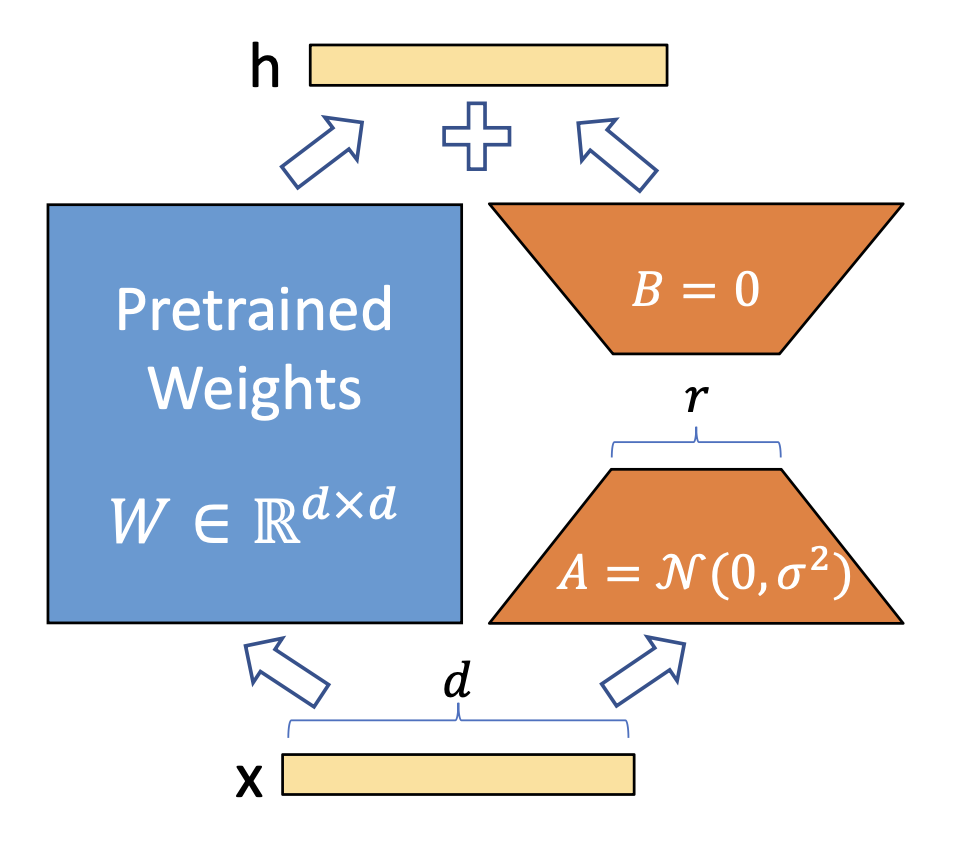
\includegraphics[width=0.4\textwidth]{5.png}
\caption{Reparametrization. Trained only A and B}
\label{fig:whisper_asr_architecture}
\end{figure}

\section{Data}
\subsection{Speech Data}

The Common Voice dataset consists of a unique MP3 and corresponding text file for Armenian language. The dataset also include demographic metadata like age, sex, and accent that can help train the accuracy of speech recognition engines.

The dataset used in this project is structured in the \texttt{DatasetDict} format provided by the \texttt{datasets} library, a high-level library designed to facilitate the processing and manipulation of datasets for machine learning applications. The dataset is organized into three splits: training, testing, and validation. Each split is created from a \texttt{.tsv} file, (which contains multiple columns detailing attributes of the data. Initially, each dataset split includes the following columns:
\begin{itemize}
    \item \texttt{client\_id}: A unique identifier for the contributor of the audio file.
    \item \texttt{path}: The relative file path to the audio file.
    \item \texttt{sentence}: The text that was spoken in the audio recording.
    \item \texttt{up\_votes}: Number of positive ratings for the clip.
    \item \texttt{down\_votes}: Number of negative ratings for the clip.
    \item \texttt{age}: The age of the speaker.
    \item \texttt{gender}: The gender of the speaker.
    \item \texttt{accents}: The accent of the speaker.
    \item \texttt{variant}: Variations of the spoken language.
    \item \texttt{locale}: The locale of the recording.
    \item \texttt{segment}: Additional segmentation information if available.
\end{itemize}

Each \texttt{.tsv} file is read into a pandas DataFrame. The paths in the DataFrame are then updated to the full paths of the audio clips. Using the \texttt{from\_pandas} method from the \texttt{datasets} library, a Dataset object is created for each DataFrame.

To focus on the primary data needed for the thesis, unnecessary columns such as \texttt{client\_id}, \texttt{up\_votes}, \texttt{down\_votes}, \texttt{age}, \texttt{gender}, \texttt{accents}, \texttt{variant}, \texttt{locale}, and \texttt{segment} are removed from each split. This simplifies the datasets to include only the \texttt{path} and \texttt{sentence} columns, making the data easier to handle and more relevant to the tasks at hand (see in Figure 6).

\begin{figure}[ht]
\centering
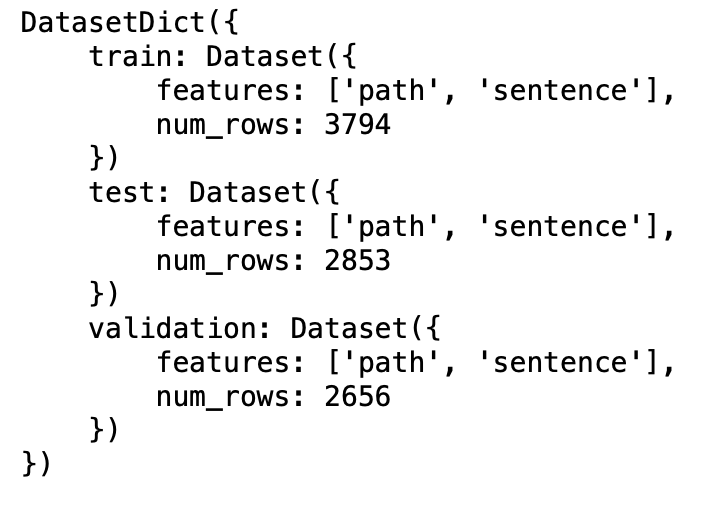
\includegraphics[width=0.5\textwidth]{4.png}
\caption{The Common Voice dataset with necessary columns}
\label{fig:whisper_asr_architecture}
\end{figure}

In the Common Voice 17.0 dataset, the train split contains 6,180 rows of data, used for training the model. Test split consists of 4,281 rows, utilized for evaluating the model’s performance after training. Validation split includes 4,214 rows, used during the model fine-tuning process to validate the results before final testing. However, for the Wav2Vec2-BERT, STT En Quartznet15x5, and STT En Citrinet 512 models, the fine-tuning is done on the train+validation splits, and the model is validated on the test split each time after a number of predefined steps.


\section{Model Fine-Tuning and Evaluation}

The listed models underwent fine-tuning using computational resources such as the NVIDIA GeForce GTX 1070 (8GB) GPU, provided by the American University of Armenia, as well as the NVIDIA A100 Tensor Core GPU (80GB) utilized through the Google Colab platform. The number of training epochs for each model can be found below:

\begin{itemize}
    \item Whisper Small with 24 hours of Common Voice dataset (Common Voice Corpus 16.1) - 25 epochs,
    \item Whisper Small with 48 hours of Common Voice dataset (Common Voice Corpus 17.0) - 25 epochs,
    \item Whisper Medium with 24 hours of Common Voice dataset (Common Voice Corpus 16.1) using LoRA - 25 epochs,
    \item Wav2Vec2 XLS-R with 48 hours of Common Voice dataset (Common Voice Corpus 17.0) - 50 epochs.
    \item Wav2Vec2-BERT with 48 hours of Common Voice dataset (Common Voice Corpus 17.0) - 10 epochs
    \item STT En Quartznet15x5 model with 48 hours of Common Voice dataset (Common Voice Corpus 17.0) -  30 epochs (frozen encoder) + 20 epochs (un-frozen encoder)
    \item STT En Citrinet 512 model with 48 hours of Common Voice dataset (Common Voice Corpus 17.0) - 90 epochs
    
    \end{itemize}

Whisper Small model was fine-tuned both on Common Voice dataset with 24 hours of recording and 48 hours of recording. The Whisper Small model was fine-tuned with the following hyperparameters:

\begin{itemize}
    \item \texttt{per\_device\_train\_batch\_size=16},
    \item \texttt{gradient\_accumulation\_steps=1},
    \item \texttt{learning\_rate=1e-5},
    \item \texttt{warmup\_steps=1},
    \item \texttt{num\_train\_epochs=25},
    \item \texttt{gradient\_checkpointing=True},
    \item \texttt{per\_device\_eval\_batch\_size=8},
    \item \texttt{predict\_with\_generate=True},
    \item \texttt{generation\_max\_length=225},
    \item \texttt{save\_strategy = "epoch"},
    \item \texttt{evaluation\_strategy = "epoch"},
    \item \texttt{logging\_strategy="epoch"},
    \item \texttt{load\_best\_model\_at\_end=True},
    \item \texttt{metric\_for\_best\_model="wer"}
    \end{itemize}

\quad \quad Whisper Medium model was fine-tuned on Common Voice dataset with 24 hours of recording using LoRA. The Whisper Medium model was fine-tuned with the following hyperparameters:

\begin{itemize}
    \item \texttt{per\_device\_train\_batch\_size=4},
    \item \texttt{gradient\_accumulation\_steps=4},
    \item \texttt{learning\_rate=1e-3},
    \item \texttt{warmup\_steps=1},
    \item \texttt{num\_train\_epochs=25},
    \item \texttt{gradient\_checkpointing=True},
    \item \texttt{per\_device\_eval\_batch\_size=2},
    \item \texttt{predict\_with\_generate=True},
    \item \texttt{generation\_max\_length=225},
    \item \texttt{save\_strategy = "epoch"},
    \item \texttt{evaluation\_strategy = "epoch"},
    \item \texttt{logging\_strategy="epoch"},
    \item \texttt{load\_best\_model\_at\_end=True},
    \item \texttt{metric\_for\_best\_model="wer"},
    \item \texttt{remove\_unused\_columns=False},  
    \item \texttt{label\_names=["labels"]}, 
    \end{itemize}
    
    \vspace{10pt}
    
    LoRA model was configured with the following hyperparameters:
    
    \begin{itemize}
    \item \texttt{r=32},
    \item \texttt{lora\_alpha=64},
    \item \texttt{target\_modules=["q\_proj", "v\_proj"]},
    \item \texttt{lora\_dropout=0.05},
    \item \texttt{bias="none"}
    \end{itemize}

Wav2vec2 XLS-R model was fine-tuned on Common Voice dataset with 48 hours of recording. The model was fine-tuned with the following hyperparameters:

\begin{itemize}
    \item \texttt{group\_by\_length=True},
    \item \texttt{per\_device\_train\_batch\_size=8},
    \item \texttt{num\_train\_epochs=50},
    \item \texttt{fp16=False},
    \item \texttt{gradient\_checkpointing=True},
    \item \texttt{learning\_rate=1e-4},
    \item \texttt{weight\_decay=0.005},
    \item \texttt{warmup\_steps=500},
    \item \texttt{greater\_is\_better=False},
    \item \texttt{lr\_scheduler\_type=SchedulerType.LINEAR},
    \item \texttt{save\_strategy = "epoch"},
    \item \texttt{evaluation\_strategy = "epoch"},
    \item \texttt{logging\_strategy="epoch"},
    \item \texttt{load\_best\_model\_at\_end=True},
    \item \texttt{metric\_for\_best\_model="wer"}
    \end{itemize}

\section{Evaluation Metrics and Results}

\subsection{Word Error Rate (WER)}

\quad \quad A typical performance indicator for automated speech recognition (ASR) systems is word error rate (WER). Since the recognised word sequence and the reference word sequence may differ in length, evaluating the effectiveness of ASR systems can be challenging. The WER operates at the word level and is derived from the Levenshtein distance. The initial step in solving this challenge is to use dynamic string alignment to align the recognised word sequence with the reference word sequence. A hypothesis known as the power law, which describes the relationship between word error rate and perplexity, can be utilised when investigating this problem. Word error rate can be calculated using the following formula:
\[
\text{WER} = \frac{S + D + I}{N} = \frac{S + D + I}{S + D + C}
\]
where:
\begin{itemize}
    \item \( S \) is the number of substitutions,
    \item \( D \) is the number of deletions,
    \item \( I \) is the number of insertions,
    \item \( C \) is the number of correct words,
    \item \( N \) is the number of words in the reference (\( N=S+D+C \)). \cite{woodard1982}
\end{itemize} 

This value indicates the average number of errors per reference word. The lower the value, the better the performance of the ASR system with a WER of 0 being a perfect score. 

\subsection{Character Error Rate (CER)}

\quad \quad An automated speech recognition (ASR) system's performance is typically measured in terms of character error rate, or CER. Though it uses characters rather than words, CER functions similarly to Word Error Rate (WER).

Character error rate can be computed as:

CER = (S + D + I) / N = (S + D + I) / (S + D + C)

where:
\begin{itemize}
    \item \( S \) is the number of substitutions,
    \item \( D \) is the number of deletions,
    \item \( I \) is the number of insertions,
    \item \( C \) is the number of correct characters,
    \item \( N \) is the number of words in the reference (\( N=S+D+C \)). \cite{morris2004}
\end{itemize}

The result of CER is not necessarily a number in the range of 0 to 1, especially when there are a lot of insertions. It is frequently linked to the proportion of characters that weren't predicted correctly. A CER of 0 represents a perfect score; the lower the value, the better the ASR system performs.

\begin{table}[ht]
    \centering
    \begin{tabular}{lcc}
        \toprule
        \textbf{Model Name} & \textbf{WER} &  \textbf{CER} \\
        \midrule
        \textbf{Whisper small} model (24 hours of data) & 42.54 & 11.03 \\
        \textbf{Whisper small} model (48 hours of data) & 36.84 & 10.45 \\
        \textbf{Whisper medium} LoRA model (24 hours of data) & 38.29&  8.24\\
        \textbf{Wav2vec2 XLS-R} model (48 hours of data) & 32.76 & 6.03\\
        \textbf{Wav2vec2-BERT} model (48 hours of data) & 12.12 & 2.17\\
        \textbf{STT En Quartznet15x5 model} (48 hours of data) & 11.75 & \\
        \textbf{STT En Citrinet 512} model (48 hours of data) & 11.23 & \\
        
        % Add more rows as needed
        \bottomrule
    \end{tabular}
    \caption{WER and CER Scores for Different Models}
    \label{tab:wer_cer_scores}
\end{table}


\section{Front-End Implementation}

The Armenian Speech Recognition initiative's user interface serves as the portal via which users interact with the system's features. Its main objectives include giving users access to various speech recognition models, transcribing audio inputs from recorded files or live recordings, and managing their transcription archives in a chat-like manner. Additionally, the front end simplifies user registration, authentication, and subscription procedures for future alerts and updates.

\subsection{Overall Structure}

The front-end architecture comprises several parts arranged into pages and reusable user interface components. The principal elements consist of:

\begin{itemize}
\item \textbf{Home Page}: Offers an overview of the program and voice recognition task options for users.
    \item \textbf{Login Page}: Provides a means for registered users to verify their identity to gain access to customized features.
    \item \textbf{Registration Page}: Facilitates account creation and provides access to platform features for new users.
    Users may establish and manage chat sessions on this page, which lets them examine and transcribe audio recordings of their previous exchanges.
    \item \textbf{Services Page}: Offers voice transcription services to those not registered or who prefer not to retain their recordings.
    \item \textbf{Reusable Components}: Consistently styled UI elements across pages, including buttons, cards, a footer, a navigation bar, and a hero section.
\end{itemize}

\subsection{Technologies and Frameworks}

The front-end uses React.js, a popular JavaScript library for building user interfaces. These were chosen for their ease of implementation and simplicity, allowing-
for efficient development of dynamic user interfaces. Additional libraries and tools used in the front-end development include:

\begin{itemize}
\item \textbf{React Router}: This component routes and navigates various application pages.
    \item \textbf{Styled Components}: Used to apply scoped CSS style to components.
     \item \textbf{Axios}: To send HTTP requests from the front end to the back end server.
    \item \textbf{React Spinners}: Used to show spinning animations or spinners while obtaining or processing data.
    \item\textbf{React Audio Voice Recorder}: An integrated feature that records user audio.
    \item \textbf{AudioBuffer-to-Wav}: Used for converting audio buffer data into WAV format.
\end{itemize}

\subsection{State Management}

React has several hooks, including \texttt{useState} and \texttt{useEffect}, that were used to handle states in a front-end application. By effectively managing component-level states and side effects, these hooks make it possible to maintain UI responsiveness and synchronization with data changes.

\subsection{Integration with Back-End}

Endpoints connected to the server's API communicate between the system's front-end and back-end parts. Axios, a popular HTTP client, mediates this interaction and typical fetching capabilities. These endpoints carry out a variety of tasks, including processing requests, submitting user input, and retrieving data. The front-end and back-end components of the application effectively communicate and share data thanks to this smooth connectivity.

\subsection{Deployment with Vercel}

Vercel was used as a front-end cloud to deploy the front-end application. An outline of the deployment procedure is provided below:

\begin{enumerate}
    \item\textbf{Setup}:  By linking the GitHub repository to a Vercel project, the project was set up to function with Vercel. 
    
    \item \textbf{Configuration}: The deployment parameters were tailored to the project specifications by using Vercel's configuration options. This covers establishing deployment hooks, creating custom domains, and defining environment variables.
    
    \item \textbf{Continuous Deployment}: When Vercel's functionality for continuous deployment is enabled, any modification made to the GitHub repository initiates a fresh deployment by default. This guaranteed that the front-end application was always up to date.
\end{enumerate}

Utilizing Vercel's robust deployment infrastructure, the front-end application was effectively deployed, allowing quick iterations, uninterrupted delivery, and smooth scalability to fulfill the requirements of the Armenian voice recognition project via this link \url{https://armenian-speech-recognition.vercel.app/}

\subsection{UI}
User-friendliness and ease of use are prioritized in the front-end's user interface (UI) design. The design seeks to minimize the learning curve for users by offering a recognizable and easy experience. This methodology furthermore enables the smooth preservation of transcription history, guaranteeing users' ability to conveniently retrieve and handle their previous engagements with the site.

\begin{figure*}[ht]
\centering
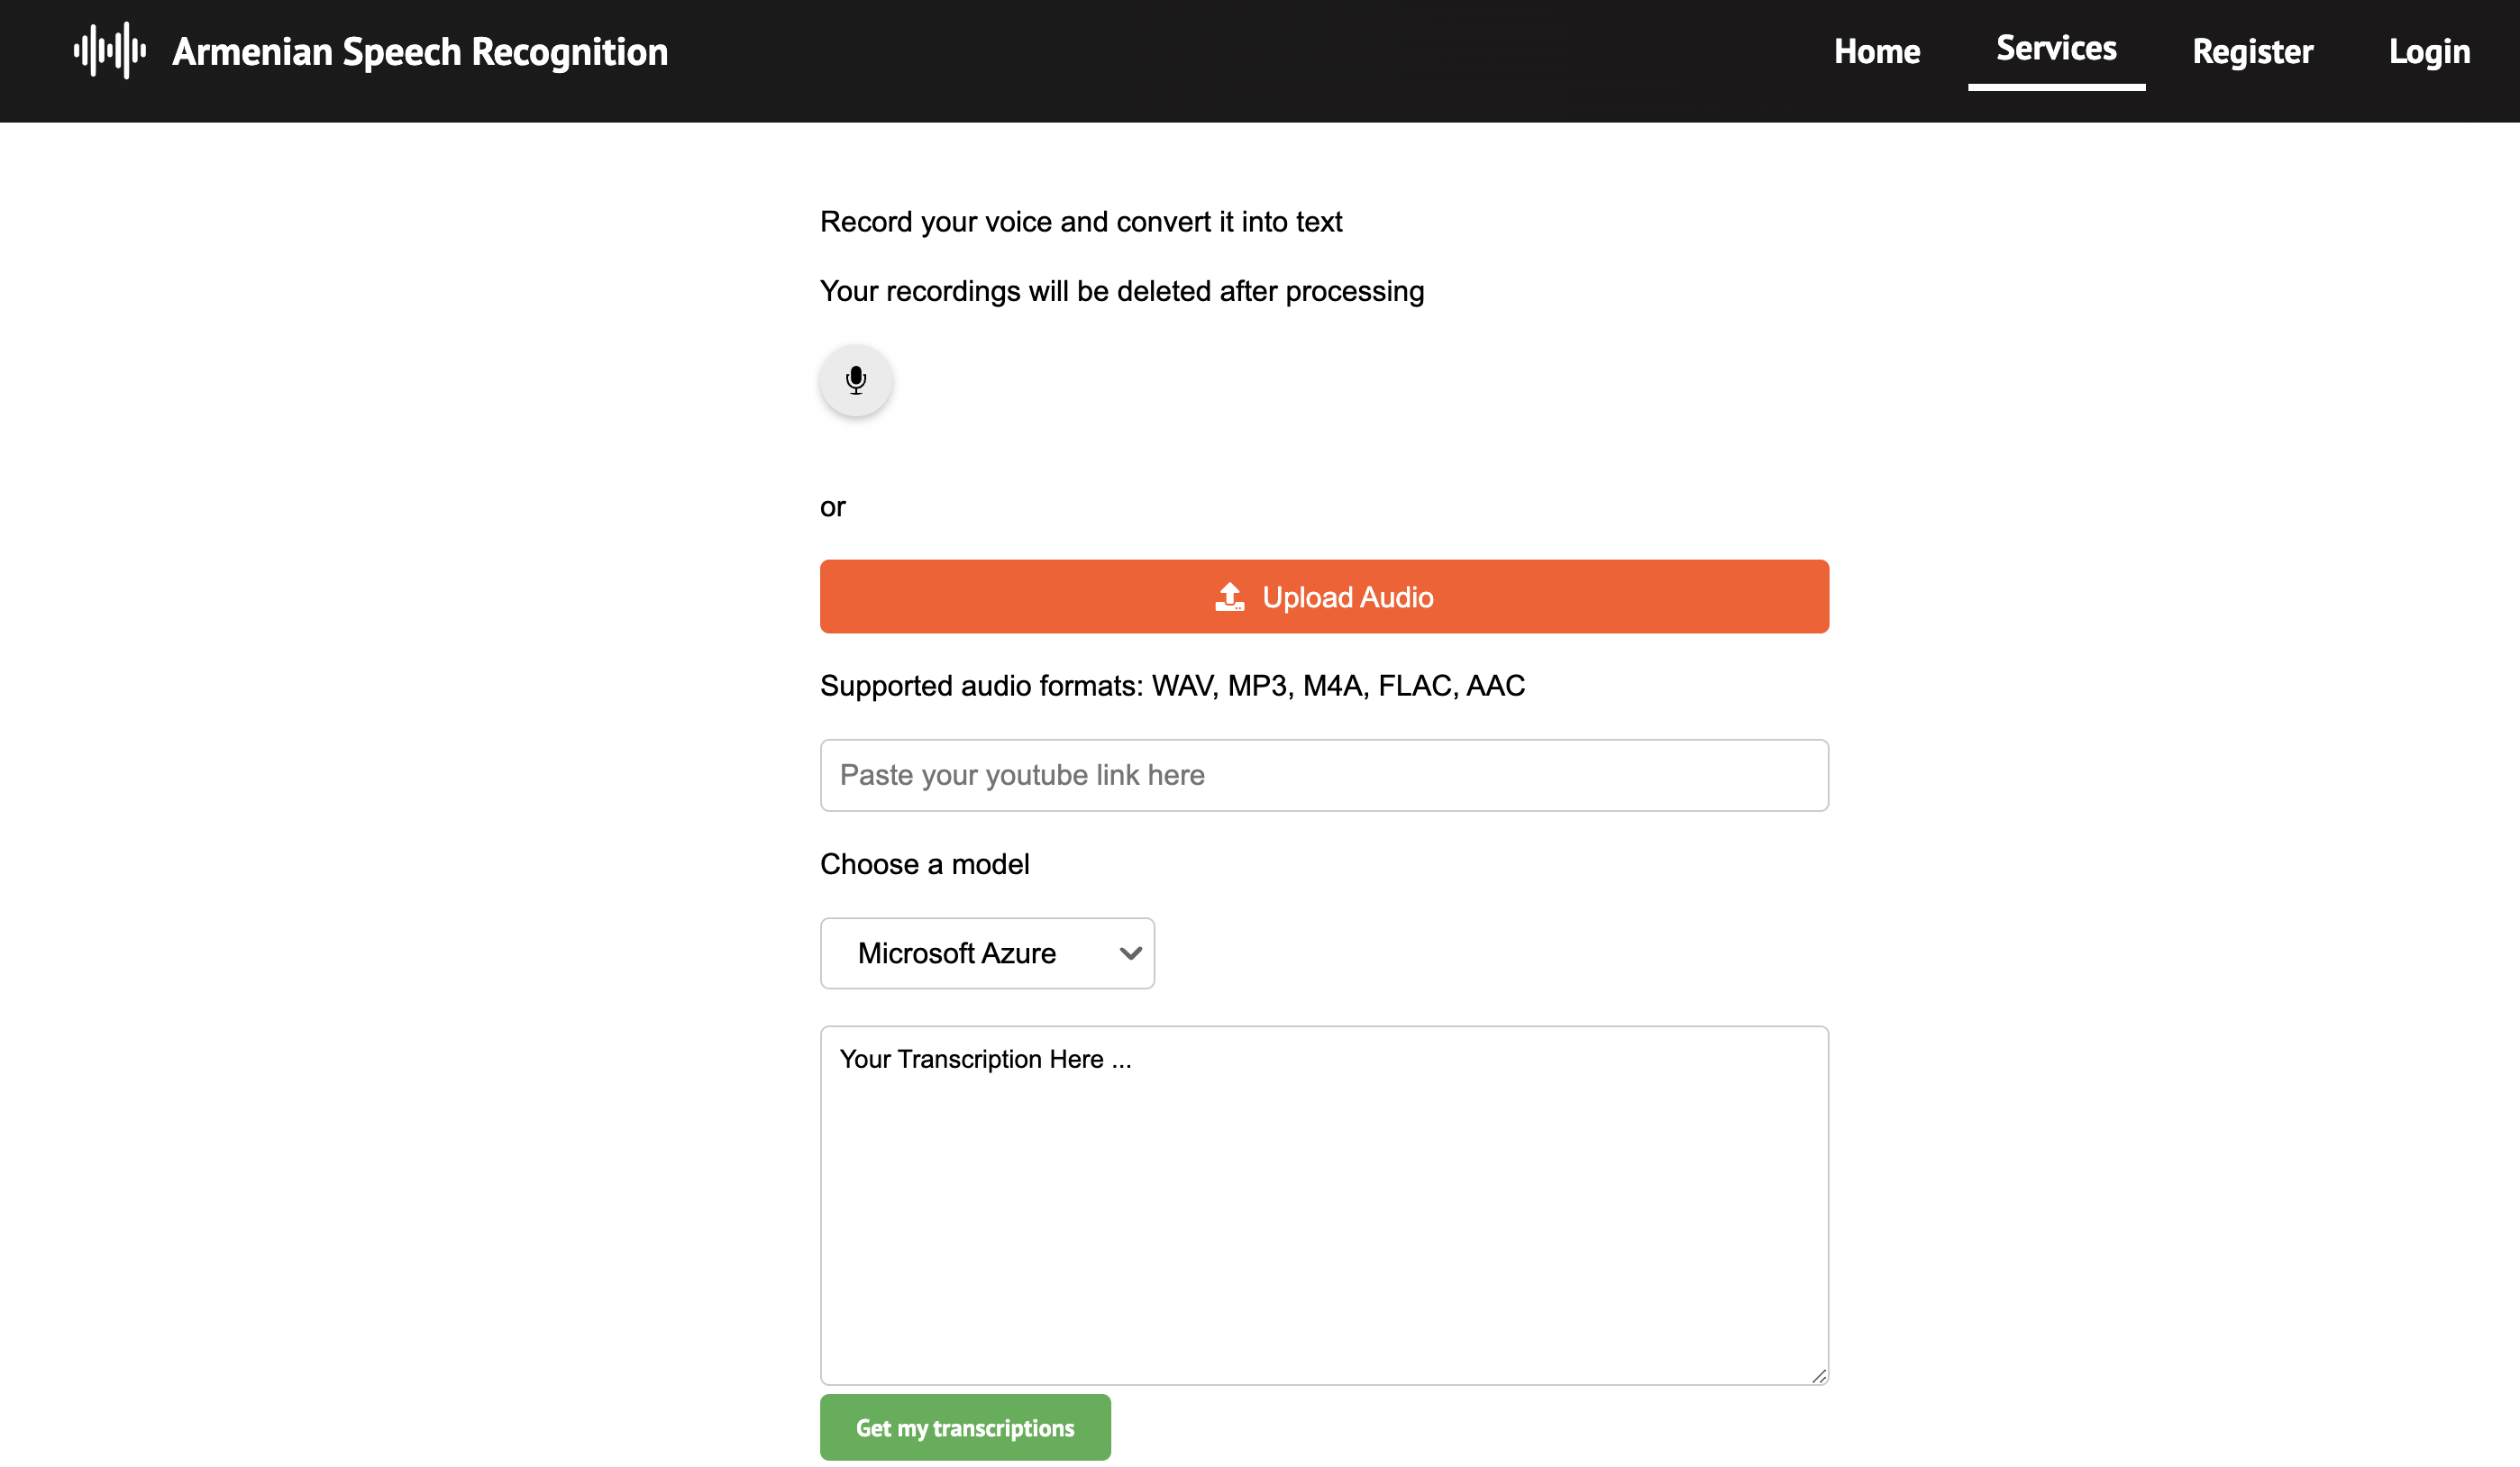
\includegraphics[width=\textwidth]{Services.png}
    \captionof{figure}{The services page for individuals who have not registered or prefer not to retain their transcription records.}
    \label{fig:ui_design_3}

\end{figure*}



\begin{center}
    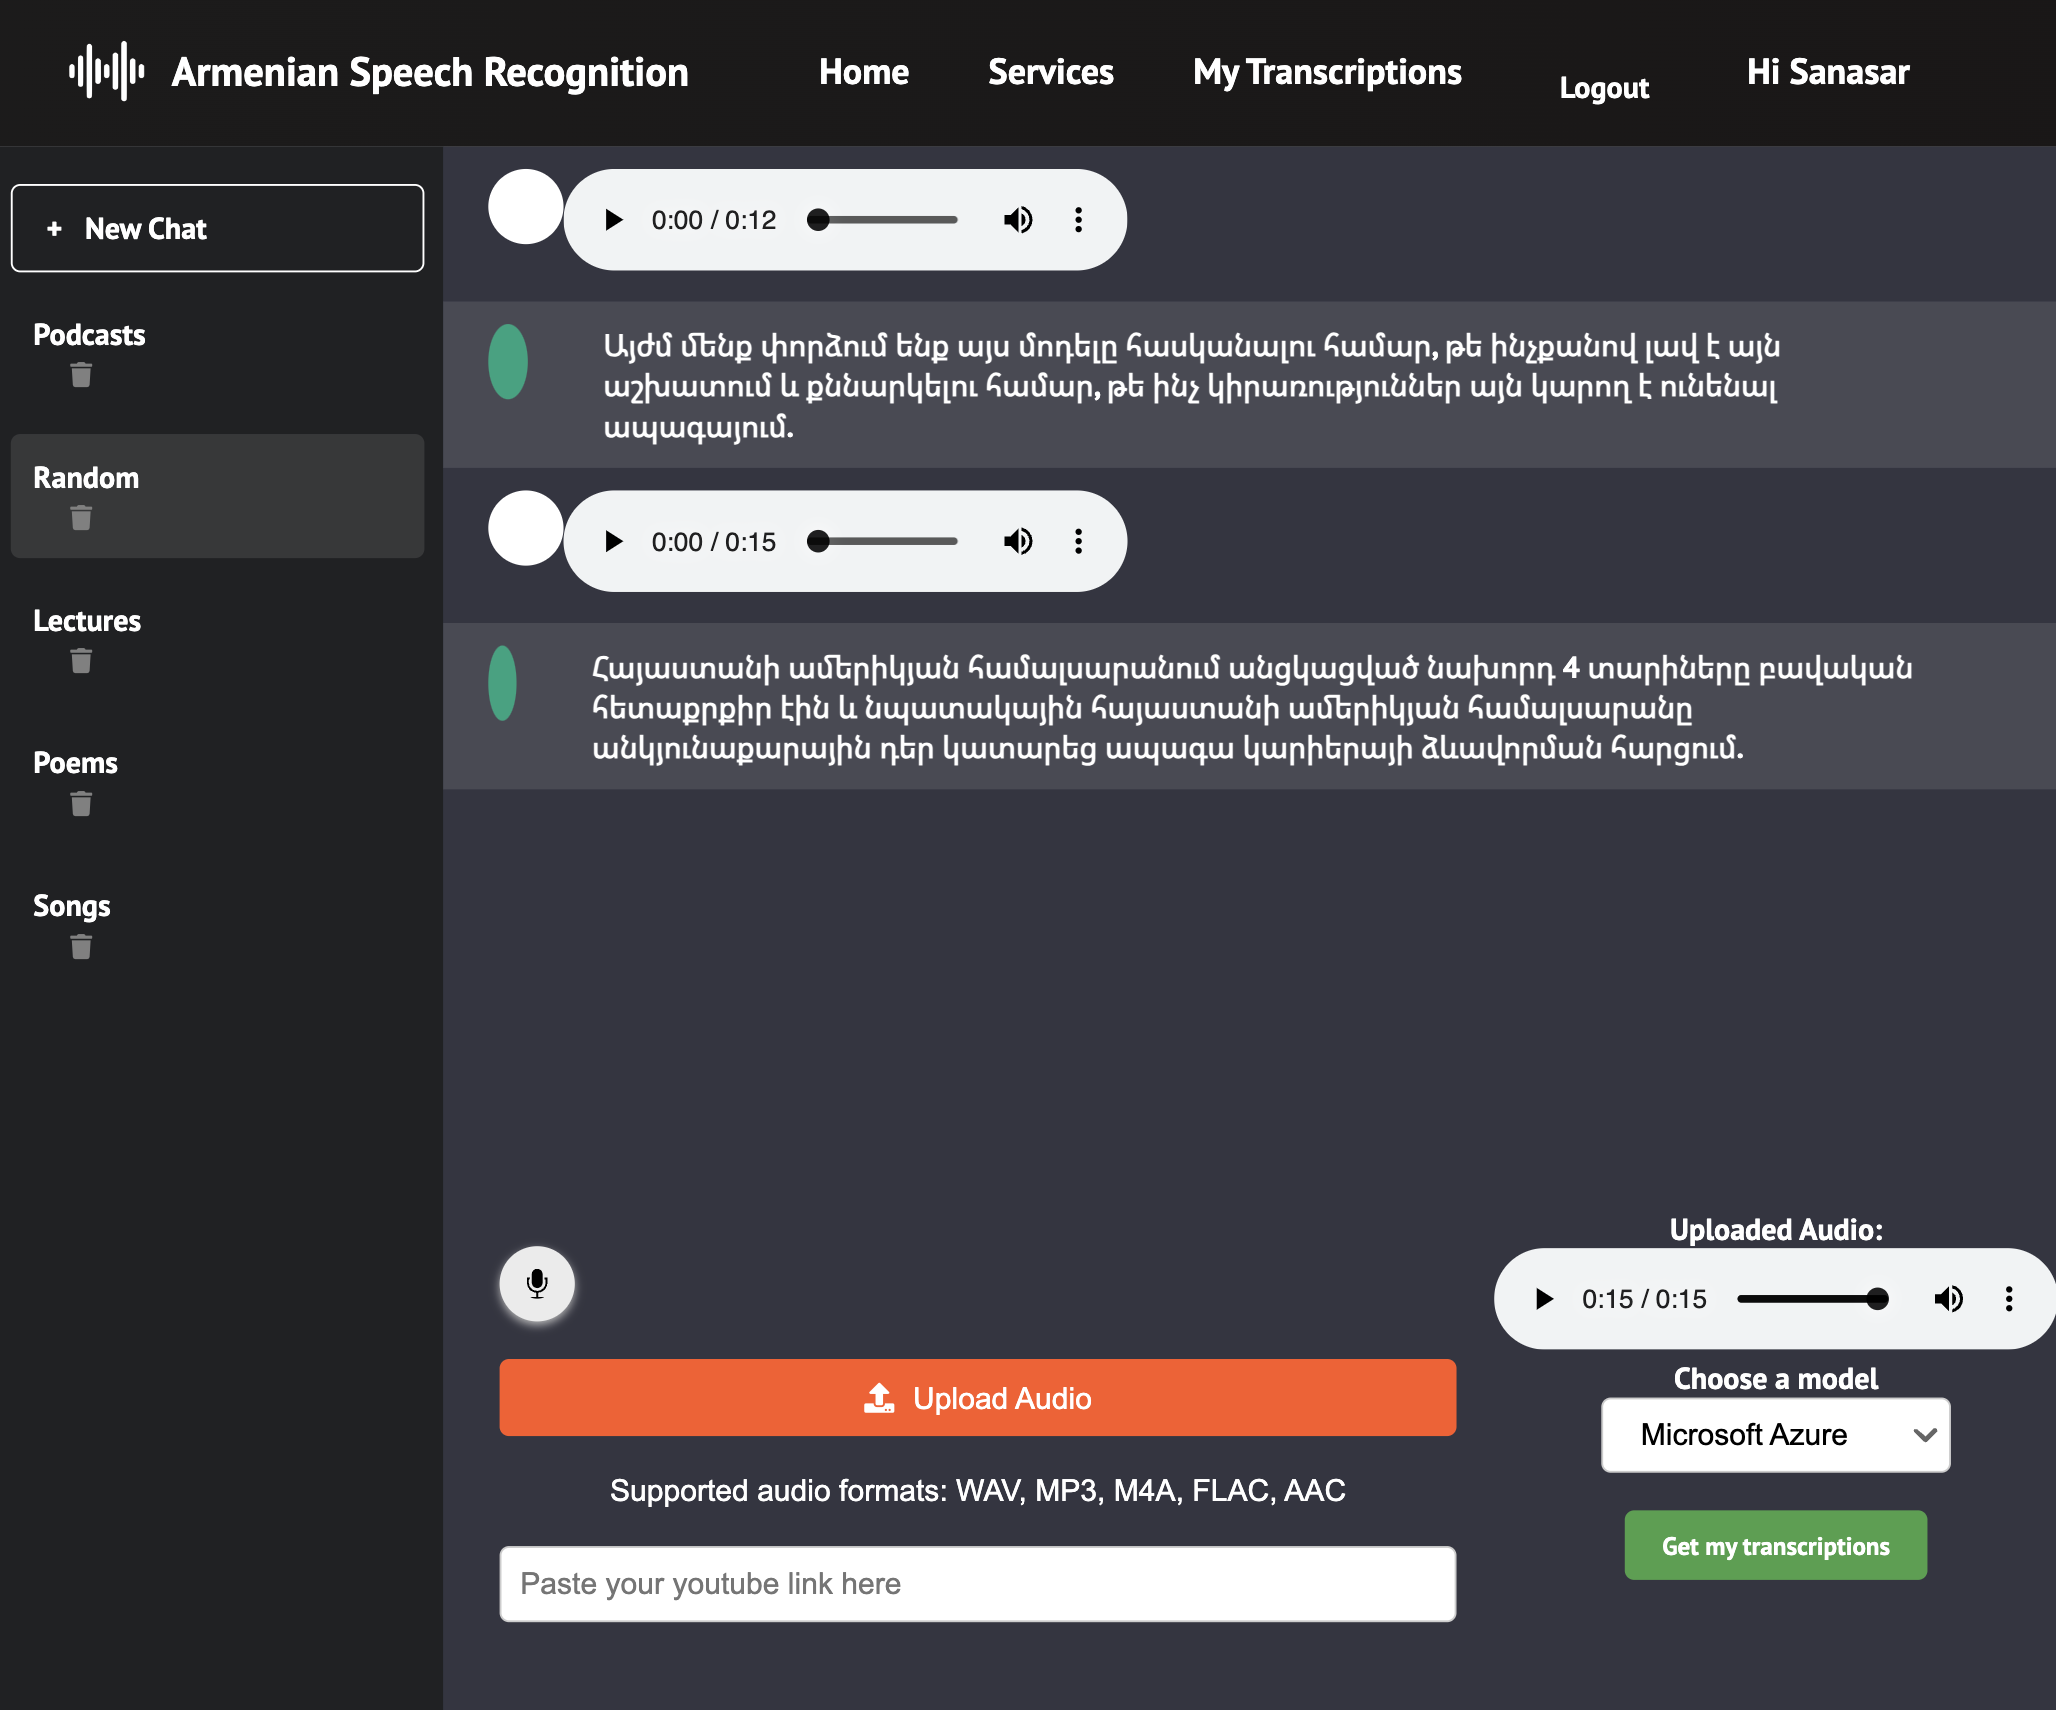
\includegraphics[width=0.5\textwidth]{RandomChat.png}
    \captionof{figure}{Screenshot of UI -- recorded audio transcription}
    \label{fig:ui_design_2}
\end{center}

\begin{center}
    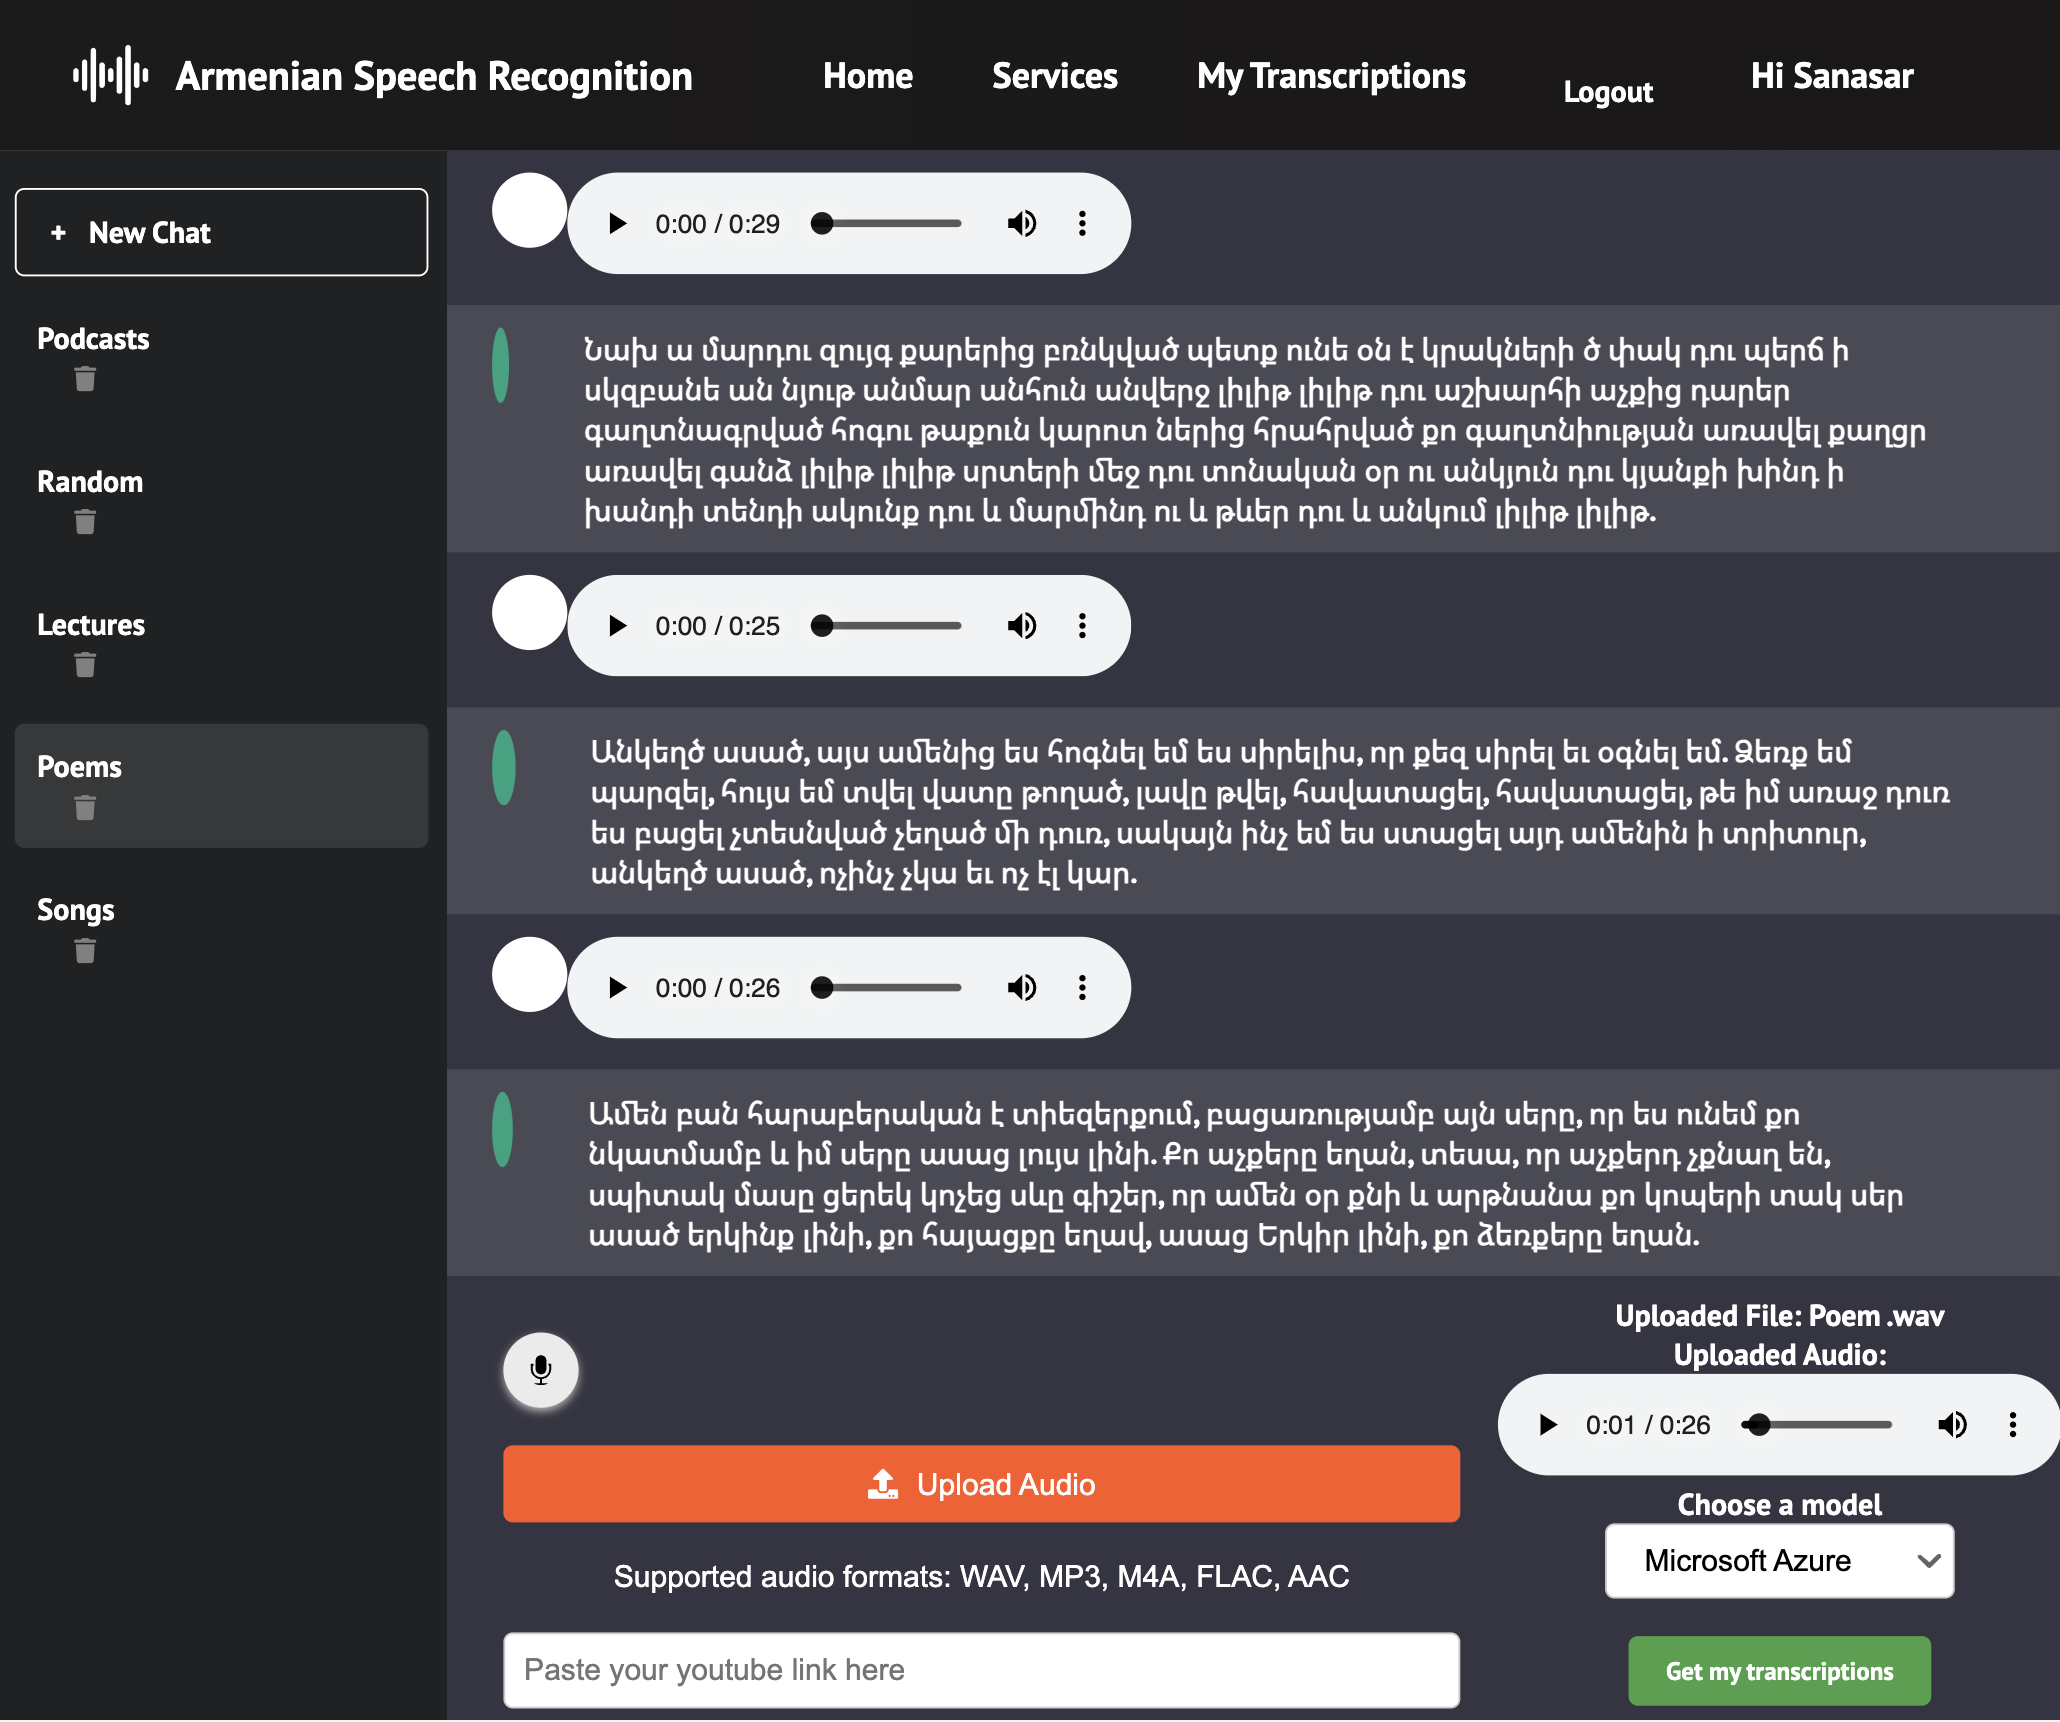
\includegraphics[width=0.5\textwidth]{PoemsChat.png}
    \captionof{figure}{Screenshot of UI -- uploaded file transcription}
    \label{fig:ui_design_1}
\end{center}




% \begin{center}
%     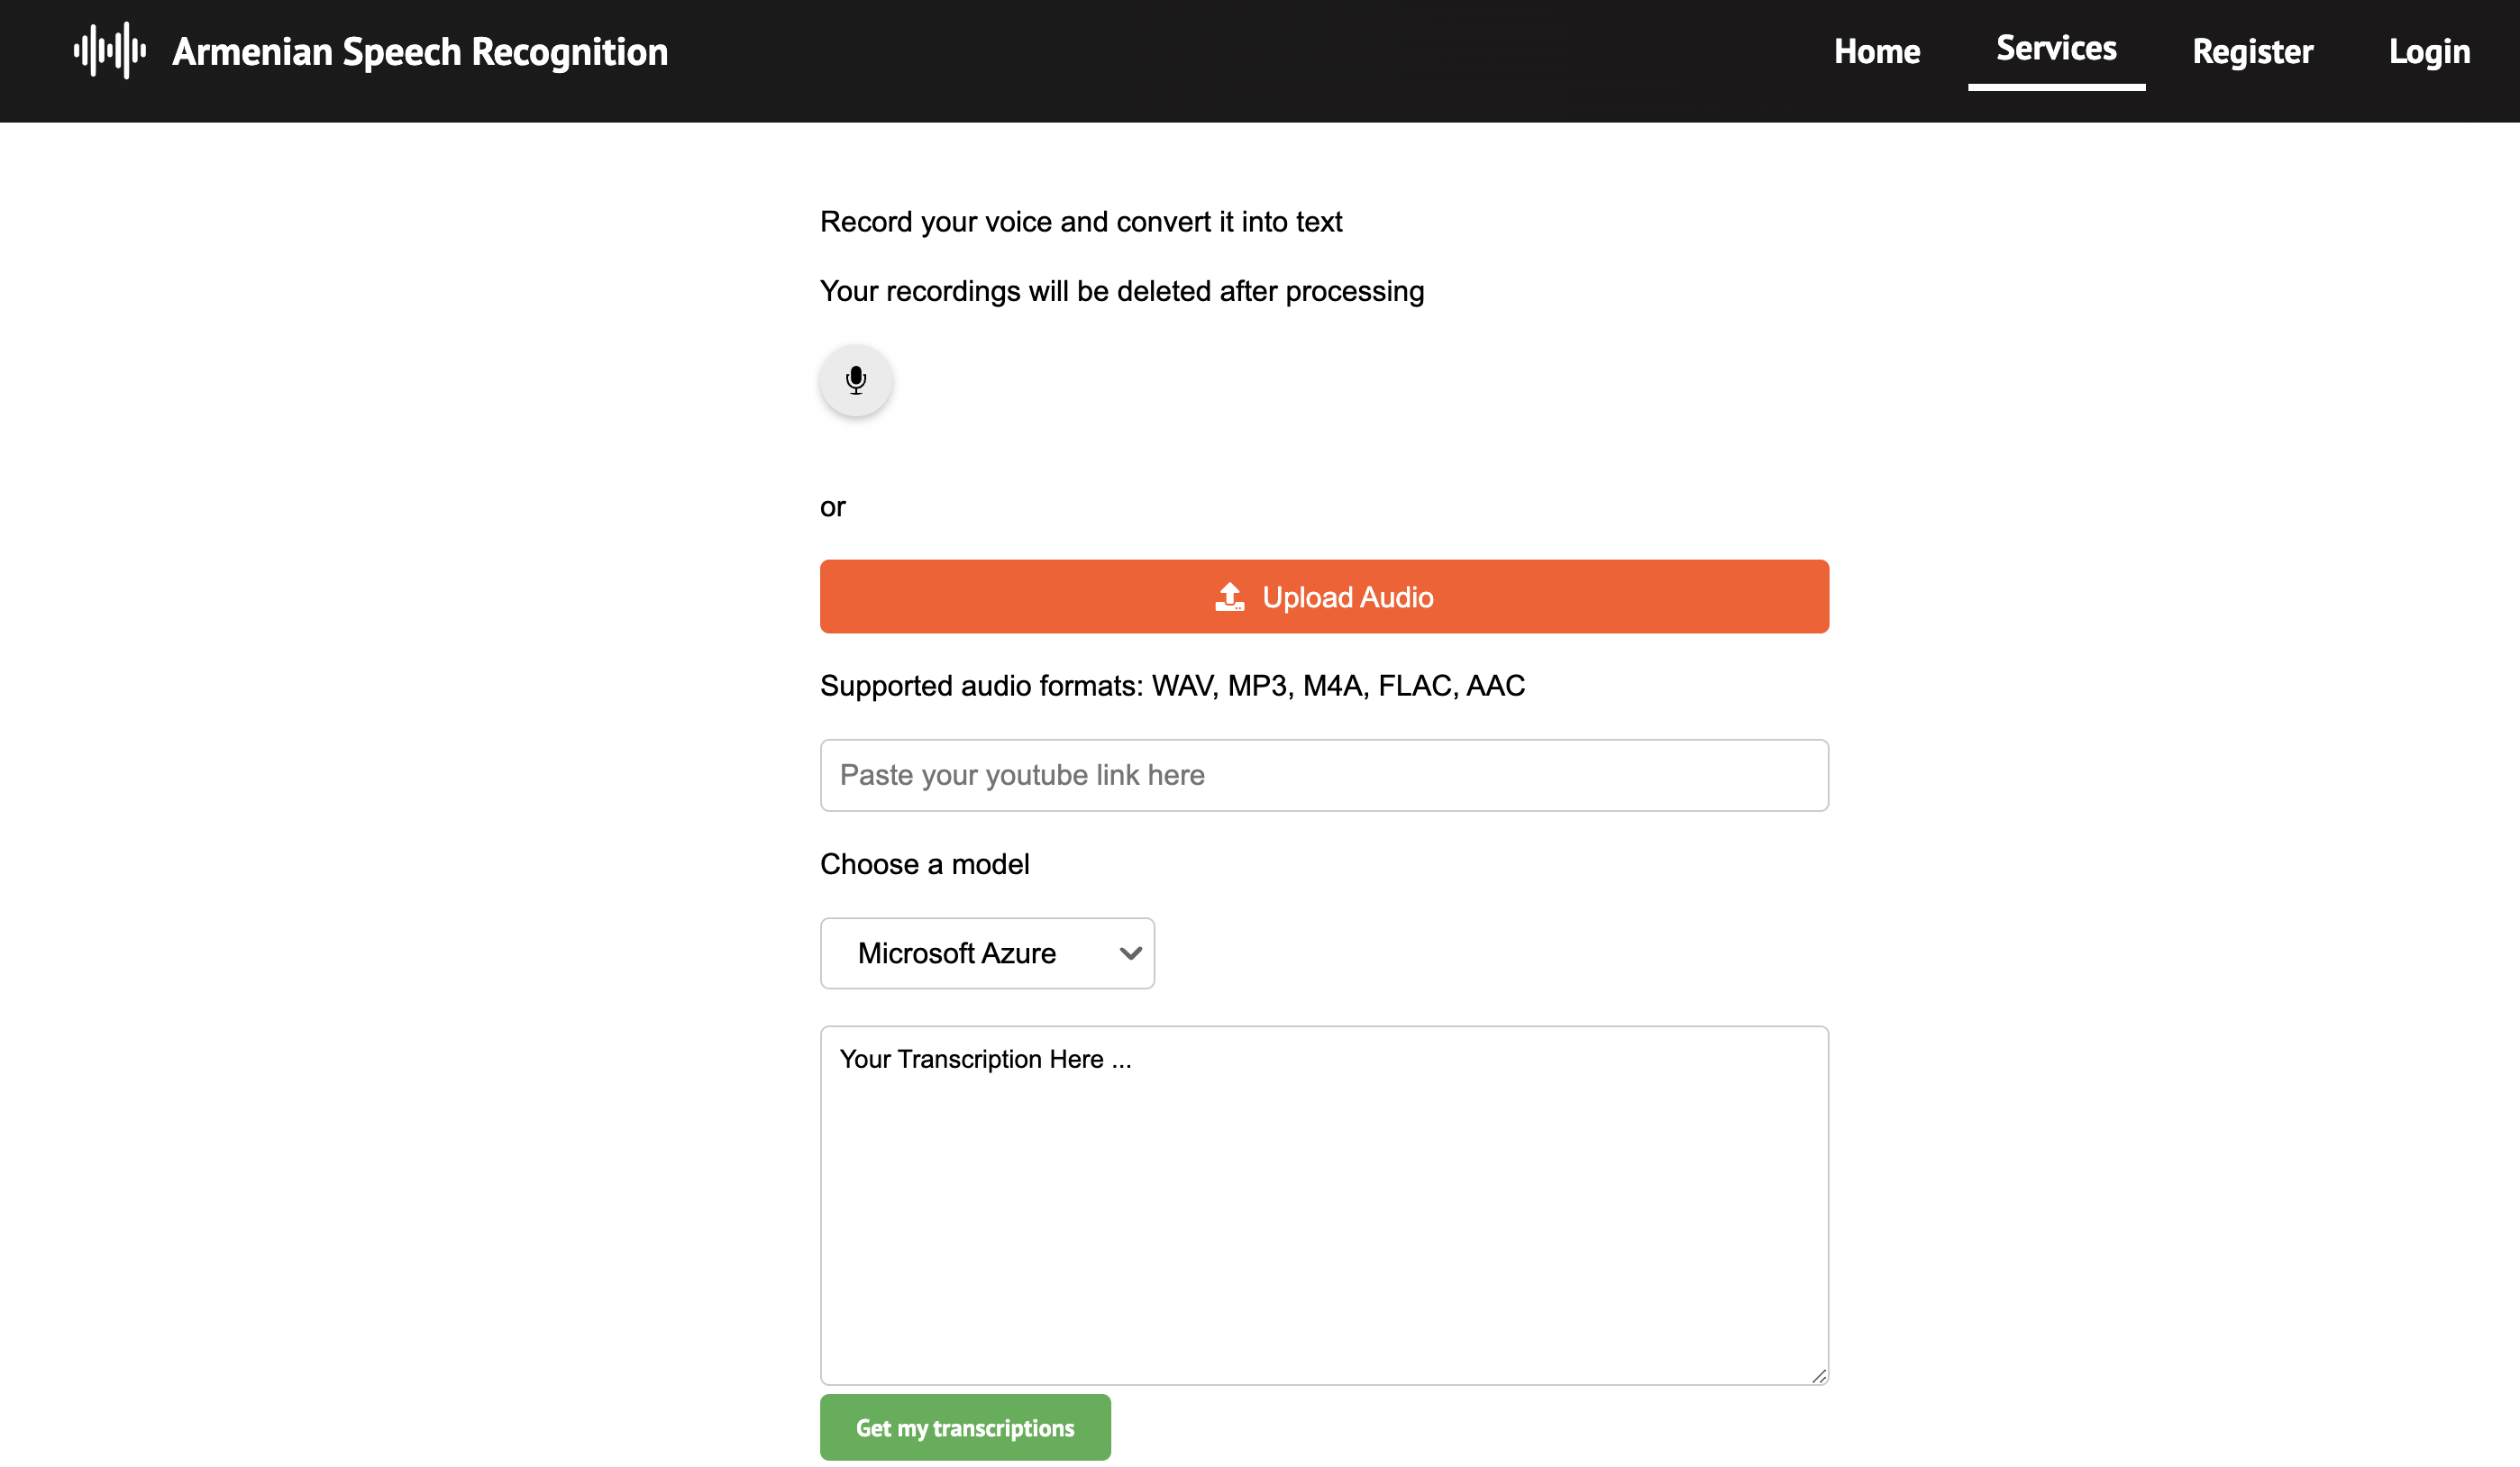
\includegraphics[width=0.5\textwidth]{Services.png}
%     \captionof{figure}{The services page for individuals who have not registered or prefer not to retain their transcription records.}
%     \label{fig:ui_design_3}
% \end{center}








\section{Back-End Development}

Java 17 and the Spring Boot framework constructed the project's back-end. With capabilities like dependency injection and integrated servers, Spring Boot makes developing Java-based web applications smoother. Maven was the build tool of choice for controlling dependencies, assembling source code, and encapsulating the program into executable artifacts.

\subsection{Back-End Architecture and Dependencies}

The project's back-end architecture uses a layered architecture pattern, which offers an organized and modular method for creating software. This architecture promotes concern separation and improves maintainability, scalability, and testability by incorporating several levels, each addressing a different part of the application's functioning.

\subsubsection{Architecture Overview}

The back-end architecture is structured into several layers, each serving distinct purposes:

\begin{enumerate}
    \item \textbf{Presentation Layer}: Managing incoming client requests, interpreting user input, and producing replies. Controller classes that define API endpoints and oversee request handling make up this layer.
    
    \item \textbf{Service Layer}: Encapsulates the application's main functionality and contains the business logic and rules relevant to it. Service classes coordinate relationships between various components, conduct business logic, and create use cases.
    
    \item \textbf{Repository Layer}: Communicates with the database and offers an abstraction over the data access layer. Repository interfaces and classes that encompass database functions, including CRUD activities, querying, and data persistence, are included in this layer.
    
    \item \textbf{Utility Layer}: Contains utility classes and helper functions, converters, and other utility functions that provide common functionality across the program.
        
    \item \textbf{Configuration Layer}: Consists of classes and configuration files that provide dependencies, environment-specific configurations, and application settings. Files, including bean configurations, security settings, and application properties, are included under this tier.
\end{enumerate}

\begin{center}
    \centering
    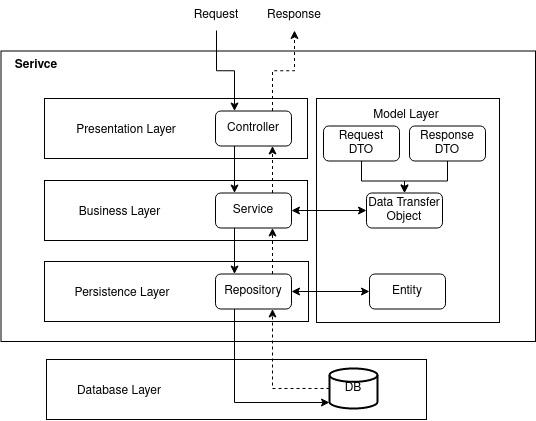
\includegraphics[width=0.5\textwidth]{LayeredArchitecture.png}
    \captionof{figure}{Back-End Architecture}
    \label{fig:backend_architecture}
\end{center}

\subsubsection{Dependencies}
To allow particular features and capabilities, the back-end depends on several dependencies, including:

\begin{itemize} \item \textbf{Spring Boot Starter Data MongoDB}: Integrates MongoDB with Spring Boot apps to streamline database access and administration.
    
    \item \textbf{Spring Boot Starter Web}: Offers all the necessary parts and setups for using Spring Boot to create web applications, such as embedded servers, HTTP request processing, and RESTful APIs.
    
    \item \textbf{Lombok}: During compilation, automatically generates getters, setters, constructors, and other common methods, reducing boilerplate code in Java classes.
\end{itemize}

These Maven-managed dependencies are automatically resolved and fetched from Maven repositories during the build process.

Following the layered architectural pattern and using these dependencies results in a well-organized back-end that benefits future development, code quality, and maintainability.



\subsection{Project Structure}

The backend project has distinct packages for each of the application's components and follows to a consistent directory structure. The primary packages consist of:

\begin{itemize}
    \item \texttt{constants}: Contains constants used throughout the application.
    \item \texttt{controller}: Contains controller classes responsible for handling HTTP requests and defining API endpoints.
    \item \texttt{model}: Contains entity classes representing database collections.
    \item \texttt{repository}: Contains repository interfaces for managing database operations.
    \item \texttt{service}: Contains service classes containing business logic.
    \item \texttt{util}: Contains utility classes.
\end{itemize}


\begin{figure*}[ht]
\centering
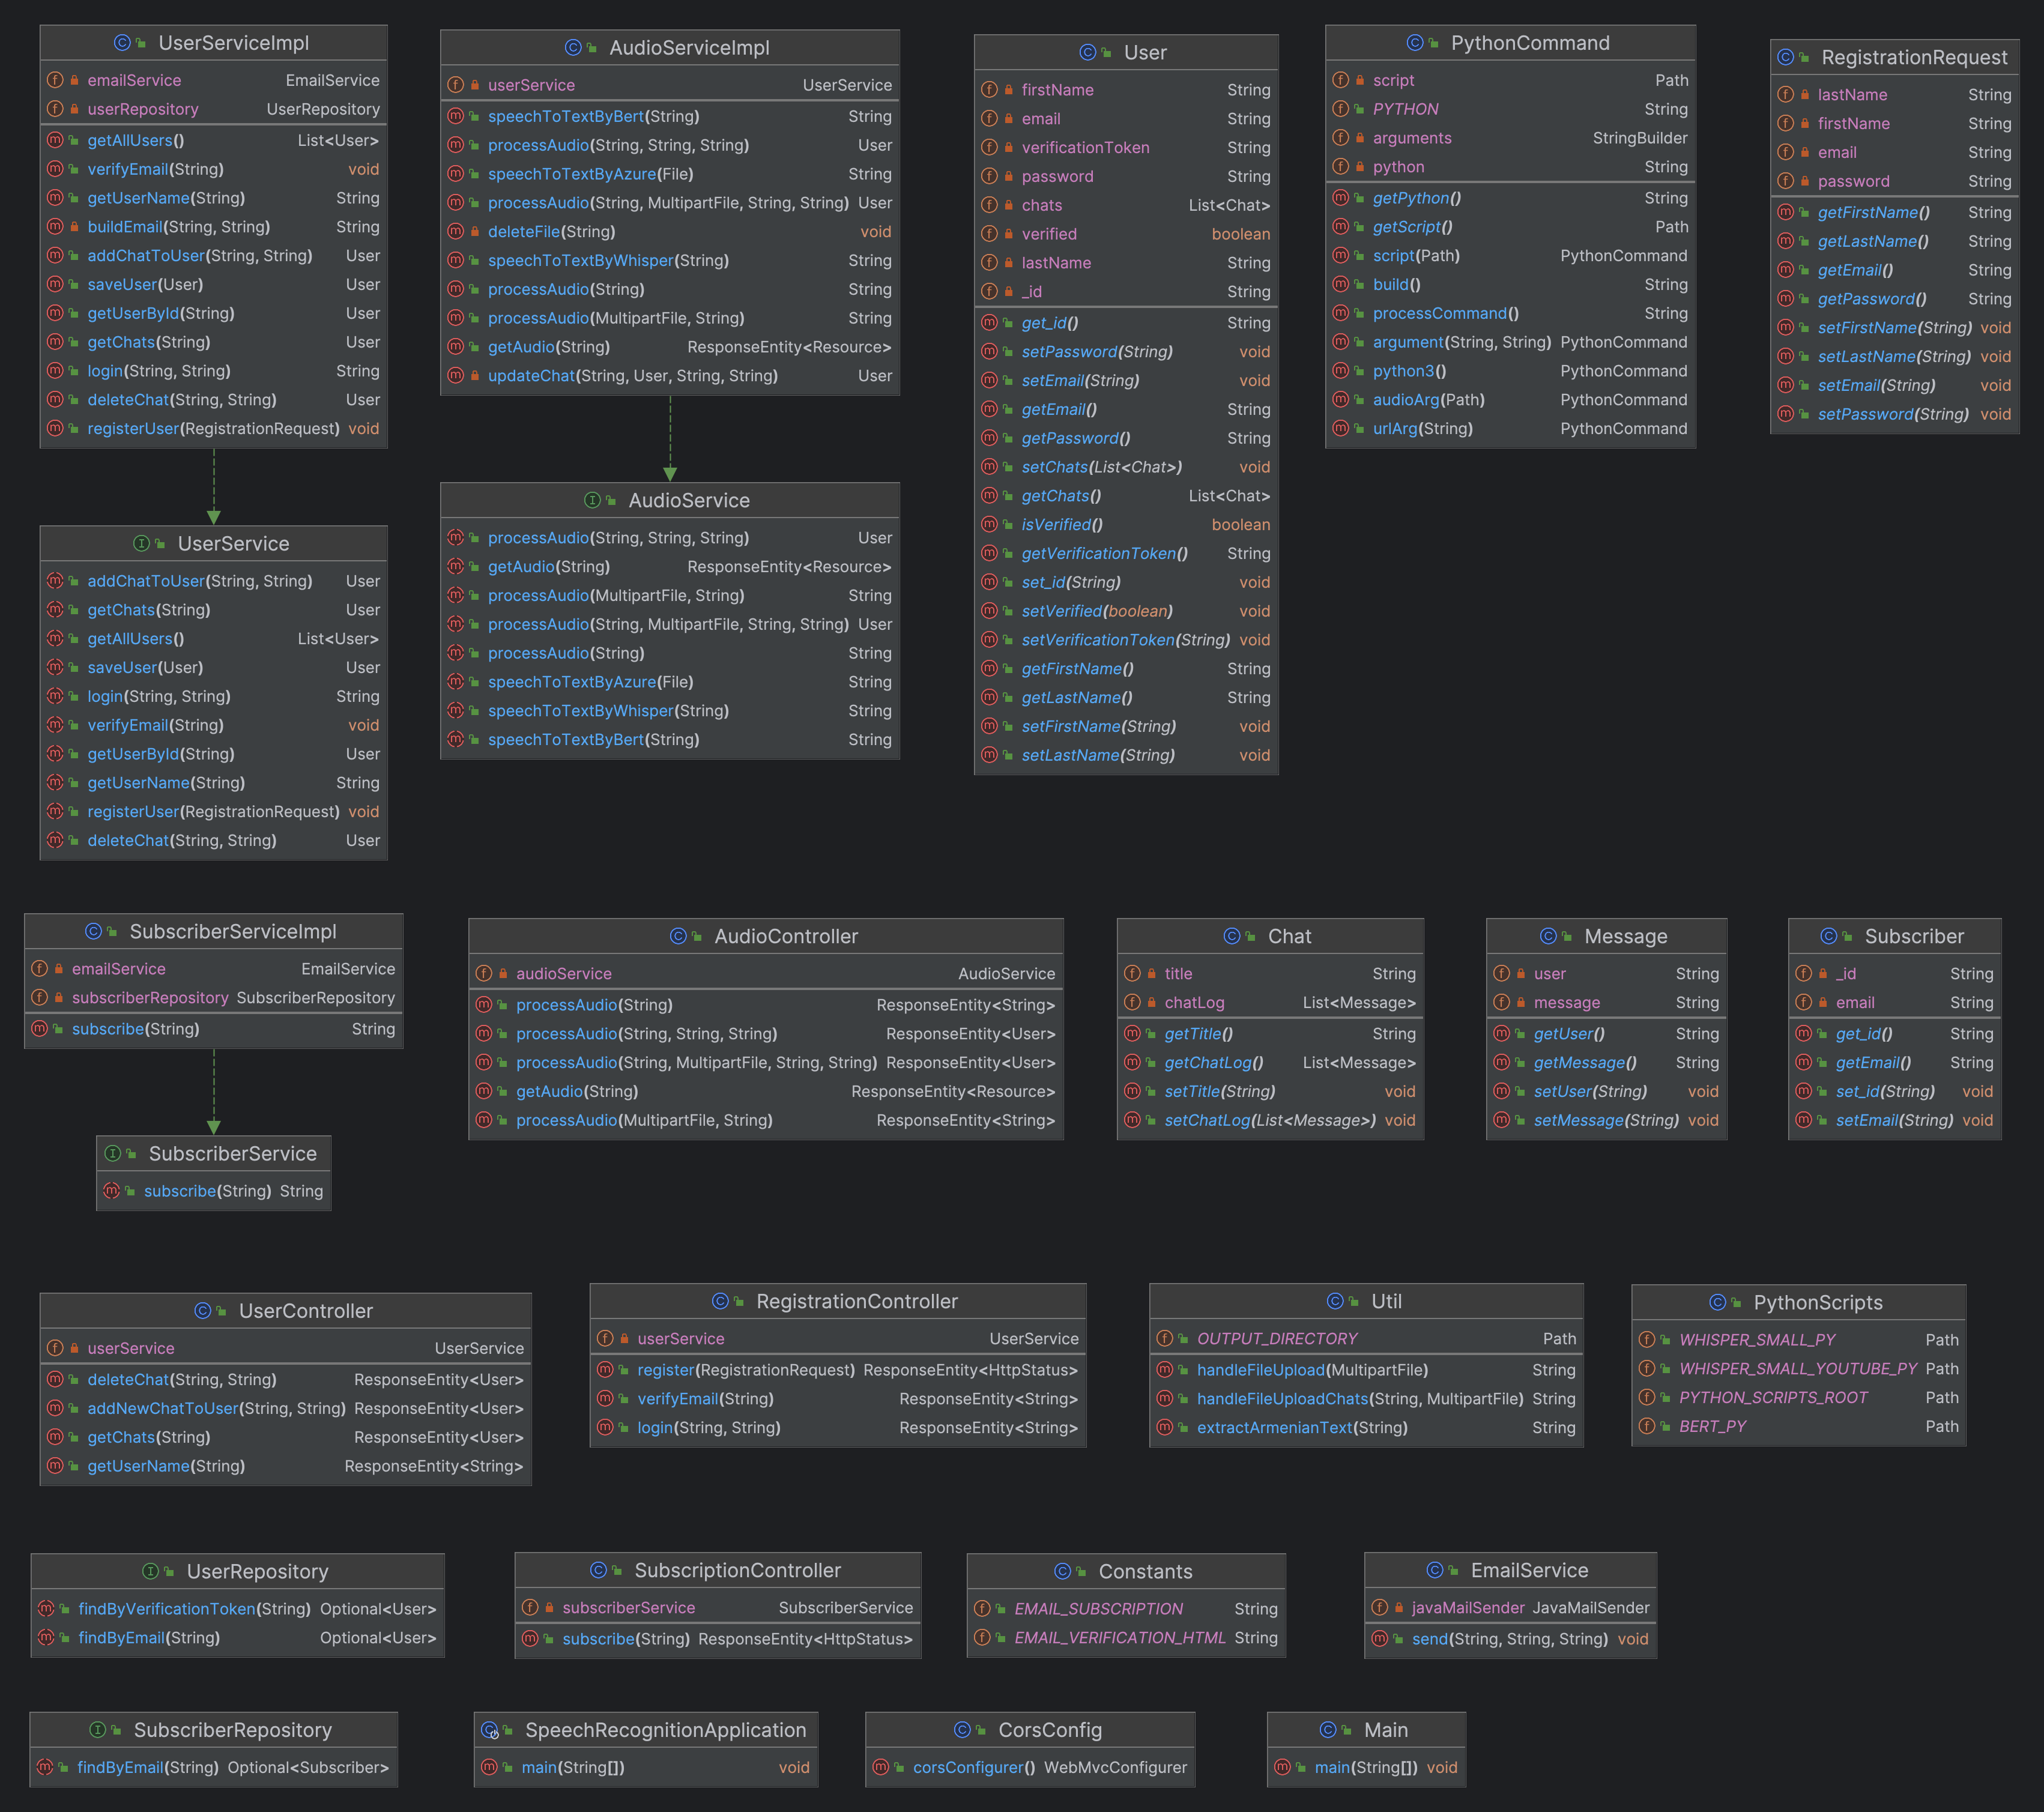
\includegraphics[width=\textwidth]{UML_Diagram.png}
    \captionof{figure}{UML Diagram}
    \label{fig:database_structure}
\end{figure*}


\subsection{Endpoints}

The backend API exposes the following endpoints:

\begin{itemize}
    \item \texttt{/users/\{userId\}}: Retrieve user information by user ID.
    \item \texttt{/users/\{userId\}/chats}: Retrieve chatLogs associated with a specific user by user ID and given chat title.
    \item \texttt{/audio/\{fileName\}}: Access audio files by file name.
    \item \texttt{/process-audio}: Process audio data for transcription.
    \item \texttt{/process-audio-link}: Process audio data from a provided YouTube link.
    \item \texttt{/process-audio-link/\{userId\}}: Process audio data from a provided YouTube link for a specific user.
    \item \texttt{/process-audio/\{userId\}}: Process audio data for a specific user.
    \item \texttt{/login}: User authentication and login.
    \item \texttt{/register}: User registration.
    \item \texttt{/verify}: User email verification.
    \item \texttt{/subscribe}: Save new subscribers to the database for future updates.
\end{itemize}


\subsection{Audio File Storage and Processing}

\subsubsection{Audio File Storage}

To compensate for database size constraints, audio files for registered users are not kept in the database directly. Rather, they are stored on the server in a different directory. For every user, the database contains simply the file names of their audio recordings. The audio files are obtained from the server directory using their file names when necessary.

\subsubsection{Audio Processing}

Processing audio data from several sources, including front-end YouTube URLs, recorded audio, and uploaded audio files, is part of the project. The relevant Python script transcribes the audio, depending on the model selected. If the Azure model is chosen, Azure is contacted via an API call to process the audio. In every other case, the Python script for the model is executed locally. Upon processing the audio, the text that has been identified is forwarded to the front end so that the user may view it. WAV, MP3, M4A, FLAC, and AAC are among the audio formats now supported by audio processing capabilities. For transcription, users can upload audio files in any of these formats.


\subsection{User Registration and Login}

To utilize the Chat-like functionality on the website, users must first register. Once registered, they can use chats and store their recordings and transcriptions for later use. Users can utilize the services page to process their audio as a one-time action, after which the audio files are deleted. 

Users must decide on a password and provide their email address to register. After registering, Java Mail Sender sends an email to the user's address with an activation link. The user may verify their email whenever convenient because the verification link does not expire after a certain time. The user cannot access their account until they click the activation link. Upon clicking the link, the database's verified state for the user changes to true, allowing a successful login.

\subsection{Password Security}

Spring's BCryptPasswordEncoder class is used to securely store registered users' passwords. This class encrypts passwords using a one-way hashing function so that decoding the original password from the hashed value is computationally impossible. Upon logging in, the password entered by the user is hashed using the same algorithm, and the resultant encoded value is cross-referenced with the hashed password saved in the database. The user can only log in successfully if the two hashed values match.



\section{MongoDB Database}

\subsection{MongoDB Atlas}

The project uses a MongoDB database housed on the extensive cloud-based database service MongoDB Atlas. The deployment and administration of databases across several cloud service providers, including AWS, Azure, and GCP, is made easier by MongoDB Atlas. MongoDB Atlas was selected mainly for its effectiveness in setting up, running, and growing MongoDB in the cloud. This made it the perfect fit for our requirements, particularly since we only keep the bare minimum of user data—such as chat names and logs, and only email addresses are kept for the subscribers' collection.

\subsubsection{Cluster Details}

This project's MongoDB cluster is housed on AWS in the Frankfurt area (eu-central-1). Version 7.0.8 of MongoDB is installed on it. The cluster offers high availability and data redundancy with three nodes as a replica set.

The cluster's backup capability is not in use at the moment. This MongoDB cluster is primarily used to store and manage data for the Armenian Speech Recognition system; hence, it is not connected to any app services.


\subsubsection{Plan Tier}

The M0 Sandbox shared tier, intended for learning and experimentation, provides resources to the MongoDB cluster. This tier offers simple setup choices and is appropriate for our small-scale project.
The M0 Sandbox tier is free, with no subscription fees required. It provides:
\begin{itemize}
    \item Storage capacity 512MB.
    \item Shared RAM and vCPU resources.
    \item The option to upgrade to dedicated clusters for full functionality and performance enhancements.
\end{itemize}

\subsection{Users Collection}

The `Users` collection stores information about registered users of the Armenian speech recognition system. Each document in the `Users` collection represents a user and contains the following fields:

\begin{itemize}
    \item \textbf{\_id:} A unique identifier for the user document.
    \item \textbf{firstName:} The first name of the user.
    \item \textbf{lastName:} The last name of the user.
    \item \textbf{email:} The email address of the user.
    \item \textbf{password:} The user's hashed password, encrypted using BCryptPasswordEncoder.
    \item \textbf{chats:} An array of chat objects containing the user's chat history.
    \item \textbf{verified:} A boolean value indicating whether the user's email address has been verified.
    \item \textbf{\_class:} The class name of the user object.
\end{itemize}

\subsection{Subscribers Collection}

The `Subscribers` collection stores information about subscribers to the Armenian Speech Recognition system. Each document in the `Subscribers` collection represents a subscriber and contains the following fields:

\begin{itemize}
    \item \textbf{\_id:} A unique identifier for the subscriber document.
    \item \textbf{email:} The email address of the subscriber.
\end{itemize}

\begin{center}
    \centering
    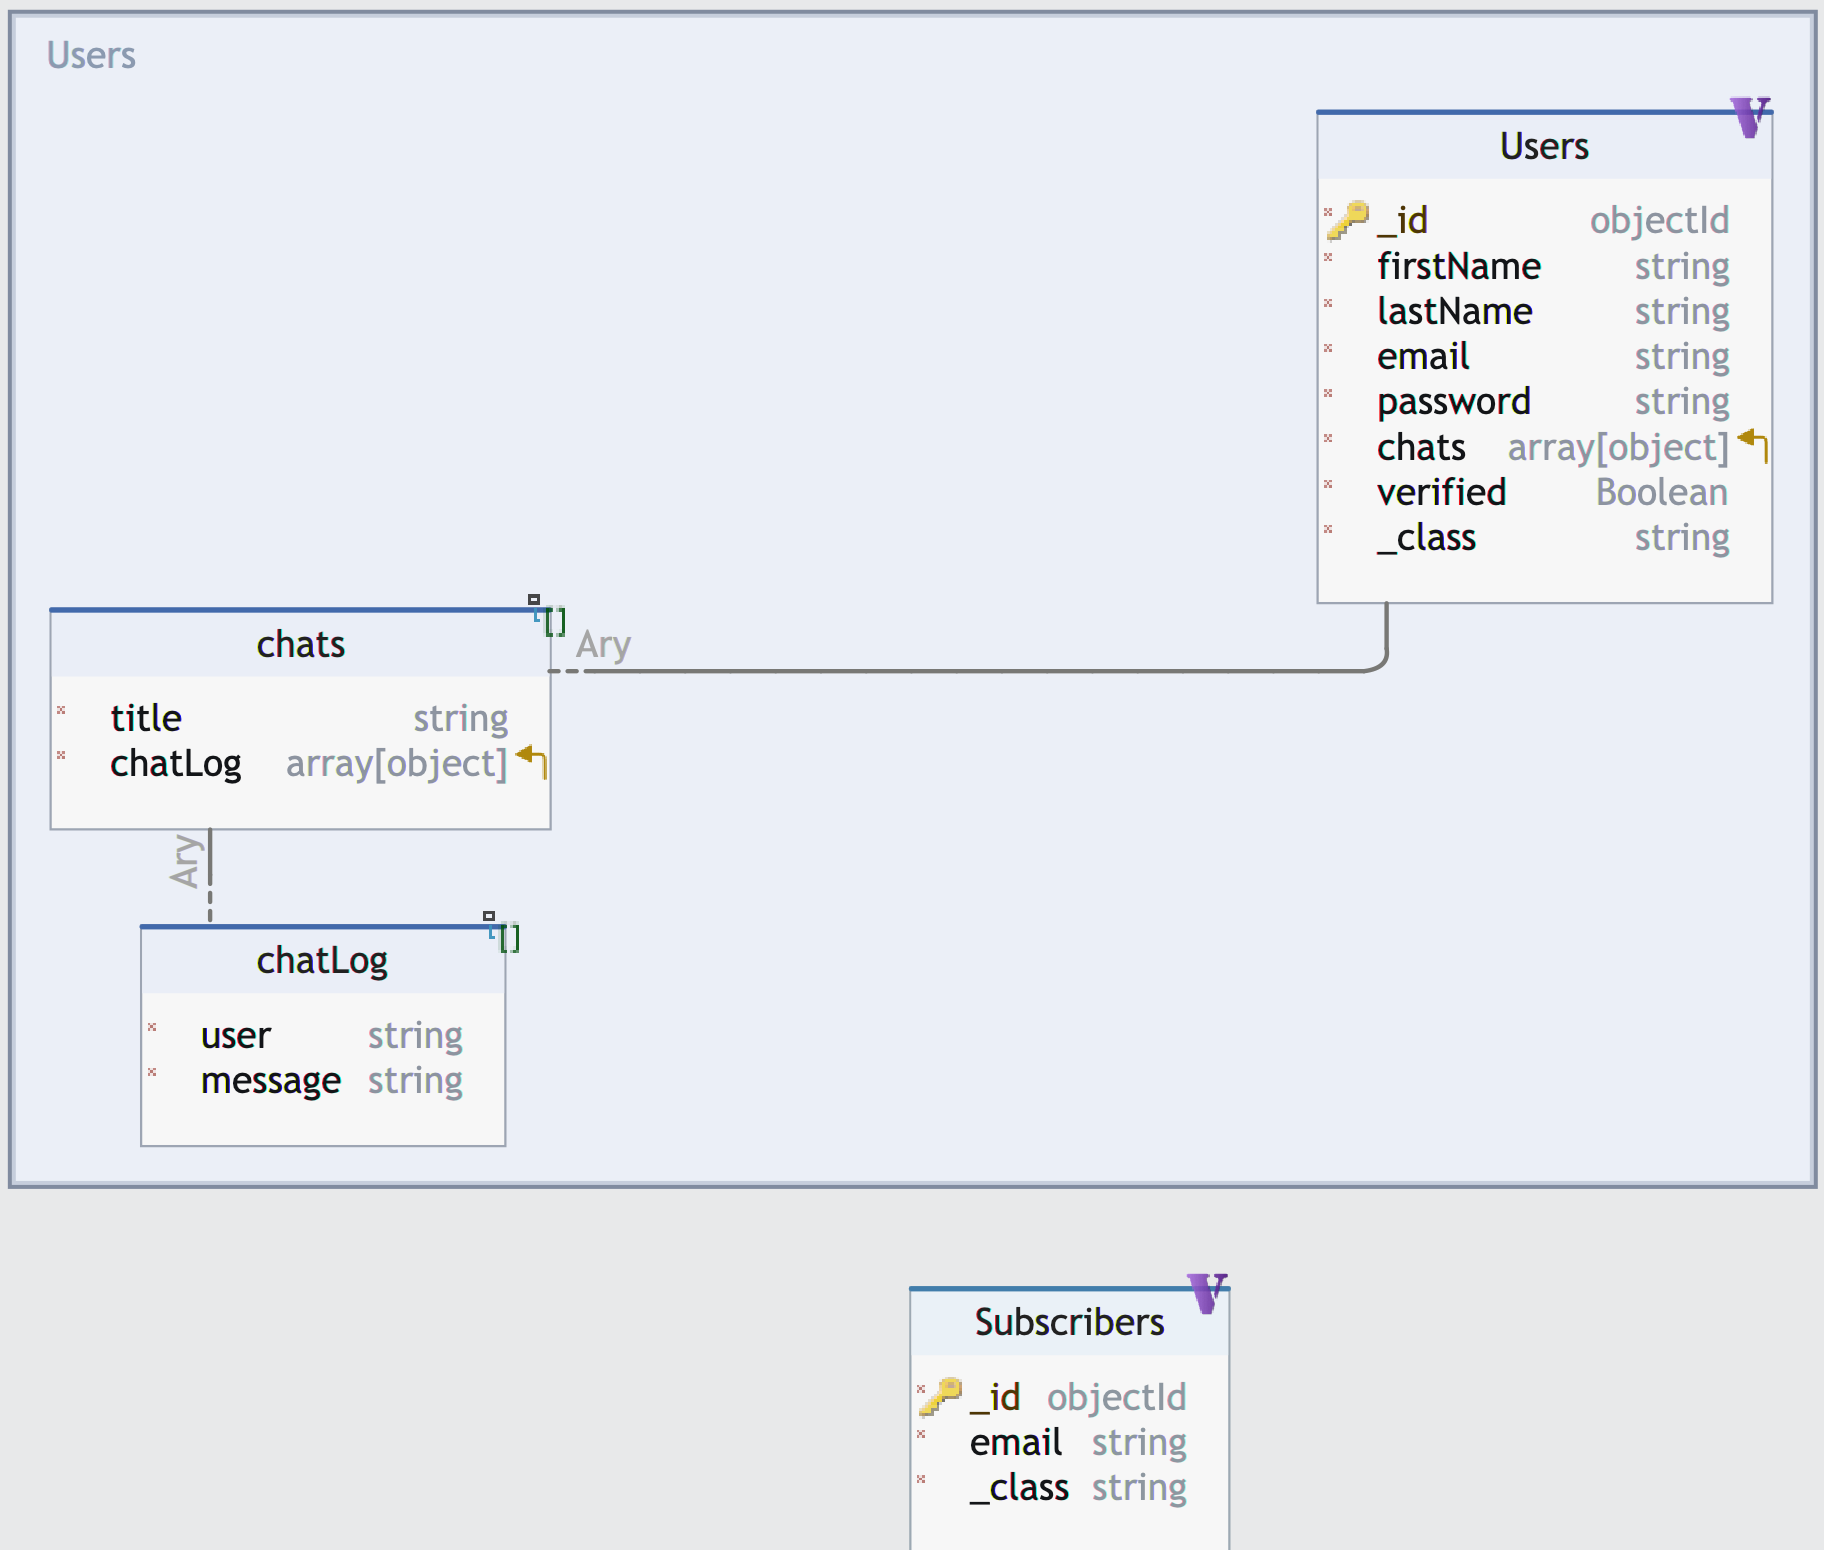
\includegraphics[width=0.5\textwidth]{DB_Structure.png}
    \captionof{figure}{Structure of the MongoDB Database}
    \label{fig:database_structure}
\end{center}




\section{Cloud Deployment}

The application's back-end server is set up on the cloud to guarantee scalability, dependability, and accessibility. There are several benefits to utilizing cloud infrastructure, such as cost-effectiveness, flexibility, and simplicity of management.
Due to restrictions in AWS free tier offers, the research resulted in the choice of Azure Cloud, which gave all new customers a \$200 credit to test out its services for 30 days. Azure was chosen due to its wide feature set and beneficial resource distribution, as the Python scripts operating in the back-end required at least two virtual CPUs and two gigabytes of RAM.



\subsubsection{Virtual Machine Configuration}

A virtual machine (VM) instance running Linux was chosen for best performance and resource allocation. With 4 vCPUs and 16 GB  of RAM, the virtual machine instance has adequate processing power and memory to run code written in Python and perform audio processing tasks effectively.

An Azure Virtual Machine (VM) instance hosting the back-end server is configured as follows:

\begin{itemize}
    \item \textbf{Operating System}: Linux (Ubuntu 22.04)
    \item \textbf{Size}: Standard D4s v3 (4 vCPUs, 16 GiB memory)
    \item \textbf{Public IP Address}: 20.52.101.91
    \item \textbf{DNS Name}: asr.germanywestcentral.cloudapp.azure.com
\end{itemize}

This VM configuration provides sufficient computational resources and network connectivity to support the back-end server, ensuring reliable performance and availability for the application.

\subsubsection{Choice of Location}

A deliberate choice was taken to strategically host the Azure Virtual Machine (VM) in the Germany West Central zone to reduce latency and maximize customer performance, especially in Armenia. To lower network latency and guarantee quicker response times for requests sent to the back-end server, we chose a data center site geographically close to the desired user base.

The decision to host the Azure virtual machine (VM) in Germany West Central is a calculated move to maximize efficiency, reduce latency, and improve user experience for anyone visiting the application from Armenia and the neighboring areas.

\section{Conclusion and Future Work}

In conclusion, this project has demonstrated effort in creating Armenian automated speech recognition (ASR) systems. Through comparative analysis, models like Wav2vec2-BERT, STT En Quartznet15x5, and others exhibit low Word Error Rates (WERs), indicating robust performance in accurately transcribing spoken language, particularly valuable for applications requiring linguistic precision and reliability.

While Whisper models show relatively higher error rates, their progress with limited training data underscores the potential for improvement through increased data exposure. The integration of LoRA conversion in Whisper models demonstrates a promising balance between resource consumption and performance enhancement, highlighting the potential for efficiency gains without excessive computational overhead.

The evolvement of Armenian ASR technologies suggests a path towards more inclusive and universally accessible systems that excel in standard benchmarks and exhibit adaptability in resource-constrained environments. Future model-building and fine-tuning advancements for Armenian ASR should prioritize integrating more capable language models for better grammatically correct outputs. 

Moreover, addressing current limitations, future research must concentrate on enhancing ASR accuracy by enabling seamless dialect recognition and supporting the stability of outputs despite acoustic variations such as background noise and audio quality discrepancies. Leveraging advanced signal processing algorithms and deeper neural network architectures aligned with human auditory perception can further refine ASR systems' ability to discern speech amidst challenging auditory conditions, ultimately advancing the practicality and effectiveness of automated speech recognition systems.


\bibliographystyle{plain}  
\bibliography{references} 

\end{document}
